\documentclass[11pt,a4paper]{article}
\usepackage[margin=24mm]{geometry}
\usepackage[T1]{fontenc}
\usepackage[utf8]{inputenc}
\usepackage[british]{babel}
\usepackage{lmodern,microtype,amsmath,amssymb,amsthm,booktabs,tabularx,graphicx,array}
\usepackage{xcolor,caption,placeins,listings,textcomp}
\definecolor{ink}{HTML}{243340}
\definecolor{figteal}{HTML}{007F86}
\definecolor{light}{HTML}{F2F5F7}
\usepackage[colorlinks=true,linkcolor=figteal,citecolor=figteal,urlcolor=figteal]{hyperref}
\usepackage{xr-hyper}
\externaldocument[S-]{build/supplementary}
\hypersetup{pdftitle={Compiling by exact queries over index sets},pdfauthor={Alberto Hern\'andez-Espinosa}}
\captionsetup{font=small,labelfont=bf}
\setlength{\parskip}{3pt}
\setlength{\emergencystretch}{3em}
\graphicspath{{generated/}}
\lstset{basicstyle=\ttfamily\footnotesize,backgroundcolor=\color{light},breaklines=true,columns=fullflexible,keepspaces=true,showstringspaces=false}
\newtheorem{proposition}{Proposition}
\newcommand{\bits}{\{0,1\}}
\newcommand{\den}[1]{[\![#1]\!]}
\makeatletter
\newcommand{\tableinput}[1]{\@@input #1 }
\makeatother
% Generated by phase2_evidence.Ledger. Do not edit.
\makeatletter
\expandafter\def\csname lv@aZeroAccHi\endcsname{0.0660}
\expandafter\def\csname lv@aZeroAccLo\endcsname{0.0251}
\expandafter\def\csname lv@aZeroAccLog\endcsname{0.0439}
\expandafter\def\csname lv@aZeroAccN\endcsname{100}
\expandafter\def\csname lv@aZeroAccRed\endcsname{4.3}
\expandafter\def\csname lv@aZeroAccTime\endcsname{0.073}
\expandafter\def\csname lv@aZeroAcclosses\endcsname{0}
\expandafter\def\csname lv@aZeroAccties\endcsname{74}
\expandafter\def\csname lv@aZeroAccwins\endcsname{26}
\expandafter\def\csname lv@aZeroClHi\endcsname{0.1194}
\expandafter\def\csname lv@aZeroClLo\endcsname{0.0592}
\expandafter\def\csname lv@aZeroClLog\endcsname{0.0882}
\expandafter\def\csname lv@aZeroClN\endcsname{100}
\expandafter\def\csname lv@aZeroClRed\endcsname{8.4}
\expandafter\def\csname lv@aZeroClTime\endcsname{7.286}
\expandafter\def\csname lv@aZeroCllosses\endcsname{12}
\expandafter\def\csname lv@aZeroClties\endcsname{35}
\expandafter\def\csname lv@aZeroClwins\endcsname{53}
\expandafter\def\csname lv@aZeroPub\endcsname{2.032760}
\expandafter\def\csname lv@bA\endcsname{0.01}
\expandafter\def\csname lv@bB\endcsname{0.1}
\expandafter\def\csname lv@bC\endcsname{1}
\expandafter\def\csname lv@effCeil\endcsname{0.819}
\expandafter\def\csname lv@effPred\endcsname{0.939}
\expandafter\def\csname lv@exAnchor\endcsname{1}
\expandafter\def\csname lv@exFree\endcsname{10}
\expandafter\def\csname lv@exMembers\endcsname{0, 2, 8, 10}
\expandafter\def\csname lv@exRangeHi\endcsname{7}
\expandafter\def\csname lv@exResult\endcsname{0, 2}
\expandafter\def\csname lv@facCat\endcsname{\ensuremath{-}0.0623}
\expandafter\def\csname lv@facCatHi\endcsname{\ensuremath{-}0.0430}
\expandafter\def\csname lv@facCatLo\endcsname{\ensuremath{-}0.0843}
\expandafter\def\csname lv@facInt\endcsname{+0.0075}
\expandafter\def\csname lv@facIntHi\endcsname{+0.0172}
\expandafter\def\csname lv@facIntLo\endcsname{\ensuremath{-}0.0030}
\expandafter\def\csname lv@facPrograms\endcsname{100}
\expandafter\def\csname lv@facTrav\endcsname{+0.0020}
\expandafter\def\csname lv@facTravHi\endcsname{+0.0070}
\expandafter\def\csname lv@facTravLo\endcsname{\ensuremath{-}0.0034}
\expandafter\def\csname lv@feAttempts\endcsname{160,000}
\expandafter\def\csname lv@feBelow\endcsname{4}
\expandafter\def\csname lv@feCaseChecks\endcsname{1,356}
\expandafter\def\csname lv@feCompletions\endcsname{819}
\expandafter\def\csname lv@feDiscrepancies\endcsname{0}
\expandafter\def\csname lv@feExhausted\endcsname{24}
\expandafter\def\csname lv@feFixtures\endcsname{12}
\expandafter\def\csname lv@feMinimum\endcsname{100}
\expandafter\def\csname lv@feRoundTrips\endcsname{564}
\expandafter\def\csname lv@feStreams\endcsname{16}
\expandafter\def\csname lv@hCOne\endcsname{b9697640e202c7cf2563ef3f11423f6cbd52403f91c897b62a6ab1b044672cfa}
\expandafter\def\csname lv@hExpCOne\endcsname{58ee75059dcbdd9f}
\expandafter\def\csname lv@hExpRZero\endcsname{74c87b69e6306359}
\expandafter\def\csname lv@hPOne\endcsname{d14bf39b450aaa5f}
\expandafter\def\csname lv@hRZero\endcsname{d0fcd441886cc5c3}
\expandafter\def\csname lv@ladFourHi\endcsname{+0.0726}
\expandafter\def\csname lv@ladFourLo\endcsname{+0.0442}
\expandafter\def\csname lv@ladFourQ\endcsname{+0.0579}
\expandafter\def\csname lv@ladFourT\endcsname{14.57}
\expandafter\def\csname lv@ladFourlosses\endcsname{0}
\expandafter\def\csname lv@ladFourties\endcsname{107}
\expandafter\def\csname lv@ladFourwins\endcsname{93}
\expandafter\def\csname lv@ladOneHi\endcsname{+0.0091}
\expandafter\def\csname lv@ladOneLo\endcsname{+0.0025}
\expandafter\def\csname lv@ladOneQ\endcsname{+0.0055}
\expandafter\def\csname lv@ladOneT\endcsname{1.17}
\expandafter\def\csname lv@ladOnelosses\endcsname{0}
\expandafter\def\csname lv@ladOneties\endcsname{182}
\expandafter\def\csname lv@ladOnewins\endcsname{18}
\expandafter\def\csname lv@ladThreeHi\endcsname{+0.0000}
\expandafter\def\csname lv@ladThreeLo\endcsname{+0.0000}
\expandafter\def\csname lv@ladThreeQ\endcsname{+0.0000}
\expandafter\def\csname lv@ladThreeT\endcsname{0.83}
\expandafter\def\csname lv@ladThreelosses\endcsname{0}
\expandafter\def\csname lv@ladThreeties\endcsname{200}
\expandafter\def\csname lv@ladThreewins\endcsname{0}
\expandafter\def\csname lv@ladTwoHi\endcsname{+0.0000}
\expandafter\def\csname lv@ladTwoLo\endcsname{\ensuremath{-}0.0028}
\expandafter\def\csname lv@ladTwoQ\endcsname{\ensuremath{-}0.0011}
\expandafter\def\csname lv@ladTwoT\endcsname{0.82}
\expandafter\def\csname lv@ladTwolosses\endcsname{2}
\expandafter\def\csname lv@ladTwoties\endcsname{198}
\expandafter\def\csname lv@ladTwowins\endcsname{0}
\expandafter\def\csname lv@lrnBoundary\endcsname{33}
\expandafter\def\csname lv@lrnEcoPrograms\endcsname{100}
\expandafter\def\csname lv@lrnEcoZero\endcsname{0}
\expandafter\def\csname lv@lrnFixtures\endcsname{30}
\expandafter\def\csname lv@lrnHam\endcsname{\ensuremath{-}0.107}
\expandafter\def\csname lv@lrnHamNeg\endcsname{30}
\expandafter\def\csname lv@lrnQueries\endcsname{1,639}
\expandafter\def\csname lv@lrnRand\endcsname{0.061}
\expandafter\def\csname lv@lrnShuf\endcsname{0.045}
\expandafter\def\csname lv@lvOne\endcsname{98.33}
\expandafter\def\csname lv@lvStd\endcsname{95}
\expandafter\def\csname lv@lvThree\endcsname{97.5}
\expandafter\def\csname lv@lvTwo\endcsname{98.75}
\expandafter\def\csname lv@mBits\endcsname{32}
\expandafter\def\csname lv@mOneSlot\endcsname{1}
\expandafter\def\csname lv@mPublic\endcsname{8}
\expandafter\def\csname lv@mTwoSlot\endcsname{2}
\expandafter\def\csname lv@mVlen\endcsname{8}
\expandafter\def\csname lv@mWords\endcsname{256}
\expandafter\def\csname lv@pOneAccepted\endcsname{18}
\expandafter\def\csname lv@pOneClassical\endcsname{1.901379}
\expandafter\def\csname lv@pOneExtraBoot\endcsname{2.362098}
\expandafter\def\csname lv@pOneExtraCl\endcsname{2.370890}
\expandafter\def\csname lv@pOneExtraFull\endcsname{2.376597}
\expandafter\def\csname lv@pOneExtraN\endcsname{100}
\expandafter\def\csname lv@pOneGain\endcsname{5.63}
\expandafter\def\csname lv@pOneImproved\endcsname{6}
\expandafter\def\csname lv@pOneReps\endcsname{15}
\expandafter\def\csname lv@pOneScore\endcsname{2.008466}
\expandafter\def\csname lv@pOneSlowBoot\endcsname{2.07}
\expandafter\def\csname lv@pOneSlowFull\endcsname{657.5}
\expandafter\def\csname lv@pOneSpeedBoot\endcsname{1.163}
\expandafter\def\csname lv@pOneSpeedFull\endcsname{2.132}
\expandafter\def\csname lv@pOneSpeedFullHi\endcsname{2.138}
\expandafter\def\csname lv@pOneSpeedFullLo\endcsname{2.127}
\expandafter\def\csname lv@pOneTests\endcsname{351}
\expandafter\def\csname lv@pOneWorkerBoot\endcsname{1.134}
\expandafter\def\csname lv@pOneWorkerFull\endcsname{1.947}
\expandafter\def\csname lv@rOneAccHi\endcsname{10.72}
\expandafter\def\csname lv@rOneAccLo\endcsname{6.86}
\expandafter\def\csname lv@rOneAccRed\endcsname{8.76}
\expandafter\def\csname lv@rOneAccTime\endcsname{0.82}
\expandafter\def\csname lv@rOneAccTimeHi\endcsname{0.97}
\expandafter\def\csname lv@rOneAccTimeLo\endcsname{0.68}
\expandafter\def\csname lv@rOneAccTimeThree\endcsname{0.817}
\expandafter\def\csname lv@rOneAcclosses\endcsname{0}
\expandafter\def\csname lv@rOneAccties\endcsname{73}
\expandafter\def\csname lv@rOneAccwins\endcsname{127}
\expandafter\def\csname lv@rOneAzeroHi\endcsname{7.74}
\expandafter\def\csname lv@rOneAzeroLo\endcsname{4.50}
\expandafter\def\csname lv@rOneAzeroRed\endcsname{6.04}
\expandafter\def\csname lv@rOneAzeroTime\endcsname{11.65}
\expandafter\def\csname lv@rOneAzeroTimeHi\endcsname{13.53}
\expandafter\def\csname lv@rOneAzeroTimeLo\endcsname{10.03}
\expandafter\def\csname lv@rOneAzerolosses\endcsname{0}
\expandafter\def\csname lv@rOneAzeroties\endcsname{98}
\expandafter\def\csname lv@rOneAzerowins\endcsname{102}
\expandafter\def\csname lv@rOneBonf\endcsname{99.17}
\expandafter\def\csname lv@rOneClHi\endcsname{12.84}
\expandafter\def\csname lv@rOneClLo\endcsname{8.38}
\expandafter\def\csname lv@rOneClRed\endcsname{10.58}
\expandafter\def\csname lv@rOneClTime\endcsname{76.20}
\expandafter\def\csname lv@rOneClTimeHi\endcsname{92.74}
\expandafter\def\csname lv@rOneClTimeLo\endcsname{62.41}
\expandafter\def\csname lv@rOneCllosses\endcsname{20}
\expandafter\def\csname lv@rOneClties\endcsname{42}
\expandafter\def\csname lv@rOneClwins\endcsname{138}
\expandafter\def\csname lv@rOneDevEffect\endcsname{+0.0663}
\expandafter\def\csname lv@rOneLearnOf\endcsname{30}
\expandafter\def\csname lv@rOneLearnZero\endcsname{0}
\expandafter\def\csname lv@rOnePubAfour\endcsname{2.088945}
\expandafter\def\csname lv@rOnePubAzero\endcsname{2.032760}
\expandafter\def\csname lv@rTwoDfsClL\endcsname{15}
\expandafter\def\csname lv@rTwoDfsClLog\endcsname{0.156}
\expandafter\def\csname lv@rTwoDfsClRed\endcsname{14.4}
\expandafter\def\csname lv@rTwoDfsClT\endcsname{39}
\expandafter\def\csname lv@rTwoDfsClW\endcsname{146}
\expandafter\def\csname lv@rTwoDfsEHi\endcsname{0.9757}
\expandafter\def\csname lv@rTwoDfsEJ\endcsname{0.959}
\expandafter\def\csname lv@rTwoDfsELo\endcsname{0.939}
\expandafter\def\csname lv@rTwoDfsET\endcsname{0.916}
\expandafter\def\csname lv@rTwoDfsEnL\endcsname{14}
\expandafter\def\csname lv@rTwoDfsEnT\endcsname{116}
\expandafter\def\csname lv@rTwoDfsEnW\endcsname{70}
\expandafter\def\csname lv@rTwoDfsHHi\endcsname{0.9997}
\expandafter\def\csname lv@rTwoDfsHJ\endcsname{0.989}
\expandafter\def\csname lv@rTwoDfsHLo\endcsname{0.978}
\expandafter\def\csname lv@rTwoDfsHT\endcsname{0.937}
\expandafter\def\csname lv@rTwoDfsHnL\endcsname{10}
\expandafter\def\csname lv@rTwoDfsHnT\endcsname{161}
\expandafter\def\csname lv@rTwoDfsHnW\endcsname{29}
\expandafter\def\csname lv@rTwoERoute\endcsname{0.80}
\expandafter\def\csname lv@rTwoHi\endcsname{+0.0460}
\expandafter\def\csname lv@rTwoJ\endcsname{0.969}
\expandafter\def\csname lv@rTwoLo\endcsname{+0.0182}
\expandafter\def\csname lv@rTwoLog\endcsname{+0.0312}
\expandafter\def\csname lv@rTwoPubCap\endcsname{2.102747}
\expandafter\def\csname lv@rTwoPubClassical\endcsname{1.901379}
\expandafter\def\csname lv@rTwoPubDfs\endcsname{2.187957}
\expandafter\def\csname lv@rTwoPubDirect\endcsname{2.008466}
\expandafter\def\csname lv@rTwoPubHeap\endcsname{2.088945}
\expandafter\def\csname lv@rTwoQRoute\endcsname{0.98}
\expandafter\def\csname lv@rTwoTime\endcsname{0.978}
\expandafter\def\csname lv@rTwoWTLL\endcsname{22}
\expandafter\def\csname lv@rTwoWTLT\endcsname{123}
\expandafter\def\csname lv@rTwoWTLW\endcsname{55}
\expandafter\def\csname lv@rTwoWorklist\endcsname{4.8}
\expandafter\def\csname lv@rTwoWorklistGate\endcsname{10.0}
\expandafter\def\csname lv@resident\endcsname{8}
\expandafter\def\csname lv@sliceMs\endcsname{2}
\expandafter\def\csname lv@sliceNodes\endcsname{2,048}
\expandafter\def\csname lv@tAccCases\endcsname{277}
\expandafter\def\csname lv@tAccPrograms\endcsname{142}
\expandafter\def\csname lv@tAdapterRows\endcsname{90}
\expandafter\def\csname lv@tAltSeedACostHi\endcsname{0.598}
\expandafter\def\csname lv@tAltSeedBCostHi\endcsname{0.597}
\expandafter\def\csname lv@tAltSeedCCostHi\endcsname{0.598}
\expandafter\def\csname lv@tAuditC\endcsname{143,585}
\expandafter\def\csname lv@tAuditD\endcsname{32,362}
\expandafter\def\csname lv@tAuditM\endcsname{18,219}
\expandafter\def\csname lv@tCFamaliasing\endcsname{0.591}
\expandafter\def\csname lv@tCFamdependency\endcsname{0.642}
\expandafter\def\csname lv@tCFammixed\endcsname{0.536}
\expandafter\def\csname lv@tCFamscalar\endcsname{0.590}
\expandafter\def\csname lv@tCFamvector\endcsname{0.521}
\expandafter\def\csname lv@tCertMedian\endcsname{31,572}
\expandafter\def\csname lv@tCost\endcsname{0.574}
\expandafter\def\csname lv@tCostFour\endcsname{0.5743}
\expandafter\def\csname lv@tCostHi\endcsname{0.598}
\expandafter\def\csname lv@tCostHiFour\endcsname{0.5978}
\expandafter\def\csname lv@tCostLo\endcsname{0.552}
\expandafter\def\csname lv@tCostLoFour\endcsname{0.5518}
\expandafter\def\csname lv@tDevCost\endcsname{0.589}
\expandafter\def\csname lv@tDevGate\endcsname{0.90}
\expandafter\def\csname lv@tDevLogJ\endcsname{\ensuremath{-}0.0173}
\expandafter\def\csname lv@tDevNodesC\endcsname{912}
\expandafter\def\csname lv@tDevNodesR\endcsname{471.5}
\expandafter\def\csname lv@tDevParity\endcsname{300}
\expandafter\def\csname lv@tDevPrograms\endcsname{100}
\expandafter\def\csname lv@tDevWTLL\endcsname{0}
\expandafter\def\csname lv@tDevWTLT\endcsname{256}
\expandafter\def\csname lv@tDevWTLW\endcsname{44}
\expandafter\def\csname lv@tDriftA\endcsname{0.567}
\expandafter\def\csname lv@tDriftB\endcsname{0.538}
\expandafter\def\csname lv@tDriftC\endcsname{0.598}
\expandafter\def\csname lv@tDriftD\endcsname{0.597}
\expandafter\def\csname lv@tExportRows\endcsname{1,248}
\expandafter\def\csname lv@tExportValid\endcsname{1,248}
\expandafter\def\csname lv@tFamilies\endcsname{5}
\expandafter\def\csname lv@tFixedMedC1\endcsname{0.187}
\expandafter\def\csname lv@tFixedMedR0\endcsname{0.362}
\expandafter\def\csname lv@tFixedPctC1\endcsname{1.07}
\expandafter\def\csname lv@tFixedPctR0\endcsname{2.41}
\expandafter\def\csname lv@tGateCost\endcsname{0.80}
\expandafter\def\csname lv@tGateQual\endcsname{1.01}
\expandafter\def\csname lv@tImport\endcsname{0.601}
\expandafter\def\csname lv@tInherited\endcsname{53}
\expandafter\def\csname lv@tJrA\endcsname{0.986}
\expandafter\def\csname lv@tJrB\endcsname{0.991}
\expandafter\def\csname lv@tJrC\endcsname{0.997}
\expandafter\def\csname lv@tKernelMax\endcsname{4.361}
\expandafter\def\csname lv@tKernelMed\endcsname{2.3649}
\expandafter\def\csname lv@tKernelMin\endcsname{0.920}
\expandafter\def\csname lv@tLossNoUnknown\endcsname{10}
\expandafter\def\csname lv@tLossPrograms\endcsname{4}
\expandafter\def\csname lv@tLossRuns\endcsname{17}
\expandafter\def\csname lv@tLossUnknownA\endcsname{0}
\expandafter\def\csname lv@tLossUnknownB\endcsname{6}
\expandafter\def\csname lv@tLossUnknownC\endcsname{7}
\expandafter\def\csname lv@tMCons\endcsname{0.7864}
\expandafter\def\csname lv@tMFamaliasing\endcsname{0.767}
\expandafter\def\csname lv@tMFamdependency\endcsname{0.900}
\expandafter\def\csname lv@tMFammixed\endcsname{0.727}
\expandafter\def\csname lv@tMFamscalar\endcsname{0.831}
\expandafter\def\csname lv@tMFamvector\endcsname{0.721}
\expandafter\def\csname lv@tMGate\endcsname{0.80}
\expandafter\def\csname lv@tMOldAdapter\endcsname{0.7638}
\expandafter\def\csname lv@tMPoint\endcsname{0.6061}
\expandafter\def\csname lv@tMReg\endcsname{0.8268}
\expandafter\def\csname lv@tMReplayOnly\endcsname{0.7650}
\expandafter\def\csname lv@tMWorkloads\endcsname{30}
\expandafter\def\csname lv@tMemMax\endcsname{1.302}
\expandafter\def\csname lv@tMemMed\endcsname{1.051}
\expandafter\def\csname lv@tMemPrograms\endcsname{30}
\expandafter\def\csname lv@tNodes\endcsname{10,000}
\expandafter\def\csname lv@tOrderC1\endcsname{0.577}
\expandafter\def\csname lv@tOrderC1Pairs\endcsname{461}
\expandafter\def\csname lv@tOrderR0\endcsname{0.572}
\expandafter\def\csname lv@tOrderR0Pairs\endcsname{539}
\expandafter\def\csname lv@tPPmax\endcsname{1.076}
\expandafter\def\csname lv@tPPmedian\endcsname{0.554}
\expandafter\def\csname lv@tPPmin\endcsname{0.264}
\expandafter\def\csname lv@tPPq10\endcsname{0.427}
\expandafter\def\csname lv@tPPq90\endcsname{0.878}
\expandafter\def\csname lv@tPPslower\endcsname{7}
\expandafter\def\csname lv@tParityMismatch\endcsname{0}
\expandafter\def\csname lv@tParityPairs\endcsname{1,000}
\expandafter\def\csname lv@tPctHi\endcsname{98.75}
\expandafter\def\csname lv@tPctLo\endcsname{1.25}
\expandafter\def\csname lv@tPerFamily\endcsname{40}
\expandafter\def\csname lv@tProcess\endcsname{0.649}
\expandafter\def\csname lv@tProgBetter\endcsname{25}
\expandafter\def\csname lv@tProgEqual\endcsname{173}
\expandafter\def\csname lv@tProgWorse\endcsname{2}
\expandafter\def\csname lv@tPrograms\endcsname{200}
\expandafter\def\csname lv@tPubC1A\endcsname{2.135}
\expandafter\def\csname lv@tPubC1B\endcsname{2.188}
\expandafter\def\csname lv@tPubC1C\endcsname{2.188}
\expandafter\def\csname lv@tPubR0A\endcsname{2.081}
\expandafter\def\csname lv@tPubR0B\endcsname{2.188}
\expandafter\def\csname lv@tPubR0C\endcsname{2.188}
\expandafter\def\csname lv@tPubSixC1A\endcsname{2.135275}
\expandafter\def\csname lv@tPubSixC1B\endcsname{2.187957}
\expandafter\def\csname lv@tPubSixC1C\endcsname{2.187957}
\expandafter\def\csname lv@tPubSixR0A\endcsname{2.081045}
\expandafter\def\csname lv@tPubSixR0B\endcsname{2.187957}
\expandafter\def\csname lv@tPubSixR0C\endcsname{2.187957}
\expandafter\def\csname lv@tPytest\endcsname{82}
\expandafter\def\csname lv@tQFamaliasing\endcsname{0.991}
\expandafter\def\csname lv@tQFamdependency\endcsname{0.995}
\expandafter\def\csname lv@tQFammixed\endcsname{0.986}
\expandafter\def\csname lv@tQFamscalar\endcsname{0.994}
\expandafter\def\csname lv@tQFamvector\endcsname{0.987}
\expandafter\def\csname lv@tQoneSeed\endcsname{980183}
\expandafter\def\csname lv@tQual\endcsname{0.991}
\expandafter\def\csname lv@tQualFour\endcsname{0.9908}
\expandafter\def\csname lv@tQualHi\endcsname{0.996}
\expandafter\def\csname lv@tQualHiFour\endcsname{0.9964}
\expandafter\def\csname lv@tQualLo\endcsname{0.985}
\expandafter\def\csname lv@tQualLoFour\endcsname{0.9846}
\expandafter\def\csname lv@tRawStdout\endcsname{9,528}
\expandafter\def\csname lv@tReps\endcsname{5}
\expandafter\def\csname lv@tResamples\endcsname{10,000}
\expandafter\def\csname lv@tSeed\endcsname{2026092802}
\expandafter\def\csname lv@tSeed980026C1J\endcsname{1,440}
\expandafter\def\csname lv@tSeed980026C1cycles\endcsname{20}
\expandafter\def\csname lv@tSeed980026C1scratch\endcsname{72}
\expandafter\def\csname lv@tSeed980026R0J\endcsname{1,280}
\expandafter\def\csname lv@tSeed980026R0cycles\endcsname{20}
\expandafter\def\csname lv@tSeed980026R0scratch\endcsname{64}
\expandafter\def\csname lv@tSeed980183C1J\endcsname{924}
\expandafter\def\csname lv@tSeed980183C1cycles\endcsname{22}
\expandafter\def\csname lv@tSeed980183C1scratch\endcsname{42}
\expandafter\def\csname lv@tSeed980183R0J\endcsname{726}
\expandafter\def\csname lv@tSeed980183R0cycles\endcsname{22}
\expandafter\def\csname lv@tSeed980183R0scratch\endcsname{33}
\expandafter\def\csname lv@tSeedHi\endcsname{980199}
\expandafter\def\csname lv@tSeedLo\endcsname{980000}
\expandafter\def\csname lv@tSubstantive\endcsname{975}
\expandafter\def\csname lv@tSummed\endcsname{0.464}
\expandafter\def\csname lv@tTerA\endcsname{0.730}
\expandafter\def\csname lv@tTerAhi\endcsname{493}
\expandafter\def\csname lv@tTerAlo\endcsname{0}
\expandafter\def\csname lv@tTerAms\endcsname{18.0}
\expandafter\def\csname lv@tTerB\endcsname{0.527}
\expandafter\def\csname lv@tTerBhi\endcsname{9,999}
\expandafter\def\csname lv@tTerBlo\endcsname{568}
\expandafter\def\csname lv@tTerBs\endcsname{0.38}
\expandafter\def\csname lv@tTerC\endcsname{0.491}
\expandafter\def\csname lv@tTerChi\endcsname{9,999}
\expandafter\def\csname lv@tTerClo\endcsname{9,999}
\expandafter\def\csname lv@tTerCs\endcsname{1.13}
\expandafter\def\csname lv@tTraces\endcsname{196}
\expandafter\def\csname lv@tWTLAL\endcsname{0}
\expandafter\def\csname lv@tWTLAT\endcsname{850}
\expandafter\def\csname lv@tWTLAW\endcsname{150}
\expandafter\def\csname lv@tWTLBL\endcsname{6}
\expandafter\def\csname lv@tWTLBT\endcsname{871}
\expandafter\def\csname lv@tWTLBW\endcsname{123}
\expandafter\def\csname lv@tWTLCL\endcsname{17}
\expandafter\def\csname lv@tWTLCT\endcsname{947}
\expandafter\def\csname lv@tWTLCW\endcsname{36}
\expandafter\def\csname lv@tWallTimeA\endcsname{0.984}
\expandafter\def\csname lv@tWallTimeB\endcsname{0.854}
\expandafter\def\csname lv@tWallTimeC\endcsname{0.755}
\expandafter\def\csname lv@tZeroNode\endcsname{5}
\expandafter\def\csname lv@tabPPmixedbroadcastCOne\endcsname{9\ensuremath{\times}16}
\expandafter\def\csname lv@tabPPmixedbroadcastCl\endcsname{9\ensuremath{\times}17}
\expandafter\def\csname lv@tabPPmixedbroadcastDi\endcsname{10\ensuremath{\times}24}
\expandafter\def\csname lv@tabPPmixedbroadcastJ\endcsname{144}
\expandafter\def\csname lv@tabPPmixedbroadcastSer\endcsname{11\ensuremath{\times}42}
\expandafter\def\csname lv@tabPPparallelmemoryCOne\endcsname{13\ensuremath{\times}40}
\expandafter\def\csname lv@tabPPparallelmemoryCl\endcsname{14\ensuremath{\times}56}
\expandafter\def\csname lv@tabPPparallelmemoryDi\endcsname{13\ensuremath{\times}40}
\expandafter\def\csname lv@tabPPparallelmemoryJ\endcsname{520}
\expandafter\def\csname lv@tabPPparallelmemorySer\endcsname{21\ensuremath{\times}128}
\expandafter\def\csname lv@tabPPscalardualchainCOne\endcsname{8\ensuremath{\times}3}
\expandafter\def\csname lv@tabPPscalardualchainCl\endcsname{9\ensuremath{\times}5}
\expandafter\def\csname lv@tabPPscalardualchainDi\endcsname{8\ensuremath{\times}3}
\expandafter\def\csname lv@tabPPscalardualchainJ\endcsname{24}
\expandafter\def\csname lv@tabPPscalardualchainSer\endcsname{12\ensuremath{\times}9}
\expandafter\def\csname lv@tabPPscalarpipelineCOne\endcsname{14\ensuremath{\times}6}
\expandafter\def\csname lv@tabPPscalarpipelineCl\endcsname{14\ensuremath{\times}6}
\expandafter\def\csname lv@tabPPscalarpipelineDi\endcsname{14\ensuremath{\times}6}
\expandafter\def\csname lv@tabPPscalarpipelineJ\endcsname{84}
\expandafter\def\csname lv@tabPPscalarpipelineSer\endcsname{18\ensuremath{\times}15}
\expandafter\def\csname lv@tabPPscalarselectsCOne\endcsname{10\ensuremath{\times}5}
\expandafter\def\csname lv@tabPPscalarselectsCl\endcsname{9\ensuremath{\times}6}
\expandafter\def\csname lv@tabPPscalarselectsDi\endcsname{9\ensuremath{\times}6}
\expandafter\def\csname lv@tabPPscalarselectsJ\endcsname{50}
\expandafter\def\csname lv@tabPPscalarselectsSer\endcsname{20\ensuremath{\times}16}
\expandafter\def\csname lv@tabPPvectoraxpyCOne\endcsname{11\ensuremath{\times}16}
\expandafter\def\csname lv@tabPPvectoraxpyCl\endcsname{10\ensuremath{\times}32}
\expandafter\def\csname lv@tabPPvectoraxpyDi\endcsname{10\ensuremath{\times}24}
\expandafter\def\csname lv@tabPPvectoraxpyJ\endcsname{176}
\expandafter\def\csname lv@tabPPvectoraxpySer\endcsname{14\ensuremath{\times}73}
\expandafter\def\csname lv@tabPPvectorbitmixCOne\endcsname{13\ensuremath{\times}24}
\expandafter\def\csname lv@tabPPvectorbitmixCl\endcsname{10\ensuremath{\times}40}
\expandafter\def\csname lv@tabPPvectorbitmixDi\endcsname{10\ensuremath{\times}40}
\expandafter\def\csname lv@tabPPvectorbitmixJ\endcsname{312}
\expandafter\def\csname lv@tabPPvectorbitmixSer\endcsname{16\ensuremath{\times}89}
\expandafter\def\csname lv@tabPPvectorreductionCOne\endcsname{12\ensuremath{\times}32}
\expandafter\def\csname lv@tabPPvectorreductionCl\endcsname{12\ensuremath{\times}40}
\expandafter\def\csname lv@tabPPvectorreductionDi\endcsname{12\ensuremath{\times}40}
\expandafter\def\csname lv@tabPPvectorreductionJ\endcsname{384}
\expandafter\def\csname lv@tabPPvectorreductionSer\endcsname{19\ensuremath{\times}137}
\expandafter\def\csname lv@tabPubSerial\endcsname{1.000000}
\expandafter\def\csname lv@weC1C\endcsname{9}
\expandafter\def\csname lv@weC1J\endcsname{144}
\expandafter\def\csname lv@weC1S\endcsname{16}
\expandafter\def\csname lv@weCapCcap\endcsname{17}
\expandafter\def\csname lv@weCapJ\endcsname{240}
\expandafter\def\csname lv@weCapLC\endcsname{9}
\expandafter\def\csname lv@weCapLS\endcsname{8}
\expandafter\def\csname lv@weCapScap\endcsname{26}
\expandafter\def\csname lv@weCatalogue\endcsname{11}
\expandafter\def\csname lv@weChildCerts\endcsname{3}
\expandafter\def\csname lv@weChildOp\endcsname{0}
\expandafter\def\csname lv@weChildVal\endcsname{2}
\expandafter\def\csname lv@weClassicalC\endcsname{9}
\expandafter\def\csname lv@weClassicalJ\endcsname{153}
\expandafter\def\csname lv@weClassicalS\endcsname{17}
\expandafter\def\csname lv@weCombDeclared\endcsname{7,873,200}
\expandafter\def\csname lv@weCombRoot\endcsname{972,000}
\expandafter\def\csname lv@weDirectphase1C\endcsname{10}
\expandafter\def\csname lv@weDirectphase1J\endcsname{240}
\expandafter\def\csname lv@weDirectphase1S\endcsname{24}
\expandafter\def\csname lv@weEdges\endcsname{7}
\expandafter\def\csname lv@weEpochs\endcsname{4}
\expandafter\def\csname lv@weHorizon\endcsname{17}
\expandafter\def\csname lv@weImprovements\endcsname{3}
\expandafter\def\csname lv@weLooksC\endcsname{3}
\expandafter\def\csname lv@weLooksR\endcsname{14}
\expandafter\def\csname lv@weNodes\endcsname{5,476}
\expandafter\def\csname lv@weOps\endcsname{8}
\expandafter\def\csname lv@wePubC1Fullcycles\endcsname{9}
\expandafter\def\csname lv@wePubC1Fullscratch\endcsname{16}
\expandafter\def\csname lv@wePubC1Shortcycles\endcsname{10}
\expandafter\def\csname lv@wePubC1Shortscratch\endcsname{16}
\expandafter\def\csname lv@wePubR0Fullcycles\endcsname{9}
\expandafter\def\csname lv@wePubR0Fullscratch\endcsname{16}
\expandafter\def\csname lv@wePubR0Shortcycles\endcsname{10}
\expandafter\def\csname lv@wePubR0Shortscratch\endcsname{17}
\expandafter\def\csname lv@weQAchosen\endcsname{16}
\expandafter\def\csname lv@weQAhi\endcsname{16}
\expandafter\def\csname lv@weQTchosen\endcsname{1}
\expandafter\def\csname lv@weQThi\endcsname{7}
\expandafter\def\csname lv@weQTlo\endcsname{0}
\expandafter\def\csname lv@weQTop\endcsname{2}
\expandafter\def\csname lv@weQTsurv\endcsname{3}
\expandafter\def\csname lv@weQone980026C\endcsname{23}
\expandafter\def\csname lv@weQone980026J\endcsname{1,840}
\expandafter\def\csname lv@weQone980026S\endcsname{80}
\expandafter\def\csname lv@weQone980183C\endcsname{22}
\expandafter\def\csname lv@weQone980183J\endcsname{968}
\expandafter\def\csname lv@weQone980183S\endcsname{44}
\expandafter\def\csname lv@weQueries\endcsname{15}
\expandafter\def\csname lv@weRootCerts\endcsname{5}
\expandafter\def\csname lv@weScaleFinalJ\endcsname{384}
\expandafter\def\csname lv@weScaleFirstJ\endcsname{480}
\expandafter\def\csname lv@weScaleNodes\endcsname{9,999}
\expandafter\def\csname lv@weScaleOps\endcsname{19}
\expandafter\def\csname lv@weSerialC\endcsname{11}
\expandafter\def\csname lv@weSerialJ\endcsname{462}
\expandafter\def\csname lv@weSerialS\endcsname{42}
\expandafter\def\csname lv@weStarterC\endcsname{11}
\expandafter\def\csname lv@weStarterJ\endcsname{462}
\expandafter\def\csname lv@weStarterS\endcsname{42}
\expandafter\def\csname lv@weStarterScore\endcsname{1.000000}
\expandafter\def\csname lv@weStepAC\endcsname{10}
\expandafter\def\csname lv@weStepAS\endcsname{17}
\expandafter\def\csname lv@weStepBC\endcsname{9}
\expandafter\def\csname lv@weStepBS\endcsname{17}
\expandafter\def\csname lv@weStepCC\endcsname{9}
\expandafter\def\csname lv@weStepCS\endcsname{16}
\expandafter\def\csname lv@weSubC\endcsname{4,440}
\expandafter\def\csname lv@weSubCerts\endcsname{1,655}
\expandafter\def\csname lv@weSubChildren\endcsname{3,001}
\expandafter\def\csname lv@weSubR\endcsname{27,874}
\expandafter\def\csname lv@weSubRatio\endcsname{0.16}
\expandafter\def\csname lv@weTimeC1\endcsname{100.4}
\expandafter\def\csname lv@weTimeC1Full\endcsname{233.5}
\expandafter\def\csname lv@weTimeC1Short\endcsname{10.4}
\expandafter\def\csname lv@weTimeClassical\endcsname{0.154}
\expandafter\def\csname lv@weTimeDirect\endcsname{441.680}
\expandafter\def\csname lv@weTimeR0\endcsname{100.5}
\expandafter\def\csname lv@weTimeR0Full\endcsname{239.7}
\expandafter\def\csname lv@weTimeR0Short\endcsname{10.4}
\expandafter\def\csname lv@weTimeSerial\endcsname{0.015}
\newcommand{\V}[1]{\ifcsname lv@#1\endcsname\csname lv@#1\endcsname\else\PackageError{ledger}{Undefined ledger value #1}{}\fi}
\makeatother

\newcommand{\ci}[2]{[#1,\,#2]}

\title{Compiling by exact queries over index sets\\[4pt]
\large A validated answer to the Luminal compiler challenge,\\and evidence for a different way of computing}
\author{Alberto Hern\'andez-Espinosa}
\date{September 2026}

\begin{document}
\maketitle

\begin{abstract}
This paper has two aims. The first is practical: to give a working, validated
answer to the Luminal compiler challenge, which asks a compiler to schedule a
straight-line program on a small very-long-instruction-word machine and to place
its values in a shared scratchpad, minimising both the number of cycles and the
scratch footprint. The second, which matters more to us, is to offer evidence
that a different way of computing is worth pursuing now that accelerators expose
every scheduling decision to the compiler and compilation is increasingly
searched or learned. In the compiler we describe, every scheduling and allocation
choice is the witness of an exact query over sets of decision indices, written as
cubes, and every later improvement is found by reopening related groups of
decisions, deleting impossible options with a replayable certificate, and
searching the remainder exactly. The index-set method is work in progress,
grounded in the author's published research on algorithmic information dynamics,
and we report the whole programme, including the stages that did not work. The final proposal, C1, makes the same decisions as its
predecessor R0 when both are given the same search work: \V{tParityPairs} of
\V{tParityPairs} paired runs on \V{tPrograms} fresh programs are identical. At
that fixed work, of \V{tNodes} search nodes, C1's complete compile call takes
\V{tCost} of R0's time (\V{lvThree}\% interval \ci{\V{tCostLo}}{\V{tCostHi}}), and at a
wall-clock allowance of \V{bB}\,s its output is not worse within the registered
margin (J ratio \V{tQual}, \V{lvThree}\% interval \ci{\V{tQualLo}}{\V{tQualHi}}). On the
eight public programs, which were visible during development, the method
scores \V{tPubSixC1B} against \V{rTwoPubClassical} for a classical list scheduler
with first-fit allocation. That gain is paid for in compile time; the classical
compiler remains far faster to compile, and on a fresh population it still wins
on some programs. We also report that, under a real clock, a faster search can end
at a worse local optimum, a form of path dependence that any anytime local search
inherits. The acceptance of C1 was a self-review.
\end{abstract}

\section{Introduction}\label{sec:intro}

Accelerators built for machine learning have returned the compiler to the
centre of performance. Their cores are frequently very-long-instruction-word
(VLIW) machines, in which several functional units issue in the same cycle and
the hardware makes no scheduling decisions of its own; every placement in time
and in memory is the compiler's responsibility~\cite{fisher1983}. At the same
time the programs to be compiled are increasingly generated rather than written,
and compilation itself is more and more often searched or learned, with neural
policies guiding exact solvers~\cite{gasse2019}. In that setting the question of
\emph{how} a compiler represents its decisions is not an implementation detail.
A representation that can state, exactly and compactly, which choices are legal,
which are better, and why an option was discarded, supports a kind of search and
a kind of explanation that a sequence of greedy commitments or a trained policy
does not.

The Luminal compiler challenge~\cite{luminal} is a small and precise instance of
this problem. A program is a list of operations in dependence order; the machine
has five engines with fixed issue capacities, latencies that delay when a result
may be read, and a scratchpad of \V{mWords} words of \V{mBits} bits in which
eight-word vectors must be aligned. The compiler must decide when each operation
issues and where each value lives, and it is scored by the geometric mean, over
programs, of how many times fewer cycles and scratch words it needs than a serial
compiler. The two decisions are coupled: packing a schedule tightly lengthens the
time during which values overlap, and packing memory tightly constrains when
values may be written.

We answer the challenge with a compiler in which every decision is the witness
of an exact query over index sets. This paper is also an argument. The index-set
method is \emph{work in progress}, built on the author's earlier published work on
algorithmic information dynamics~\cite{hernandez2019aid,hernandez2021aid}, and
the Luminal machine is a controlled setting in which to ask whether the method
earns its keep against conventional engineering. We therefore report the whole
programme and not only its last stage: the external benchmarks, our first and
second versions, the intermediate stages and ablations, the final proposal, and
the attempts that failed.

\paragraph{Contributions.}
\begin{enumerate}
\item A compiler whose first answer is built entirely from exact index-set
queries (Section~\ref{sec:index}) and whose improvement phase reopens related
windows of decisions, confines each question to the region where a strict
improvement can exist, deletes impossible options with replayable certificates
and searches exactly (Section~\ref{sec:c1}).
\item A shared branch state that lets each search node reuse the facts derived at
its parent while reproducing its predecessor's certificate stream in the same
order; its decisions are identical at equal work on every tested input, and it is
measurably faster (Section~\ref{sec:results}).
\item A worked example that runs every compared method on one public program and
renders what each one actually did (Section~\ref{sec:worked}).
\item A complete account of the measured gains, costs, losses and negative
results, with each number tied to its comparator, population and interval
(Sections~\ref{sec:results} and~\ref{sec:negative}, and Supplementary
Section~\ref{S-sec:ledger}).
\end{enumerate}

\paragraph{Four kinds of evidence.}
The final round produced evidence of four kinds, which we keep apart
throughout. (a)~A historical registered result: a pre-registered cost model
predicted a conservative ratio of \V{tMReg} against a gate of \V{tMGate} and
stopped the round with NO\_JUSTIFIED\_MECHANISM; review later found a scope defect
in one of its terms. (b)~A post-hoc development forecast after that defect was
corrected, of \V{tMCons} (conservative) and \V{tMPoint} (point); it is neither a
measurement nor an interval. (c)~A kernel-only replay of captured propagation
work, with a median speed-up of \V{tKernelMed} over \V{tMWorkloads} workloads
(range \V{tKernelMin} to \V{tKernelMax}); it is not a compiler speed-up. (d)~Real
compiler measurements: a development stage on \V{tDevPrograms} programs and a
confirmation on \V{tPrograms} fresh programs. Only the confirmation is
inferential.

\section{The machine and the objective}\label{sec:machine}

The experiment pins the challenge repository at a fixed revision~\cite{luminal}.
Inputs are straight-line operations in single-assignment dependence order, with
static buffer ranges and supplied test cases. Each operation must be emitted
exactly once; there is no rewriting, spilling or extra movement. The load, scalar
and vector engines may each issue \V{mTwoSlot} operations per cycle and the store
and flow engines \V{mOneSlot}. If operation $i$ produces an argument of $j$, then
$t_j\geq t_i+\ell_i$, where $\ell_i$ is the latency of $i$. Overlapping memory
accesses to one buffer keep their source order when at least one of them is a
store.

For a value $v$ written by operation $p(v)$, its lifetime is the inclusive
interval $I_v=[b_v,e_v]$ with $b_v=t_{p(v)}+\ell_{p(v)}$ and $e_v$ the latest of
$b_v$ and the issue cycles of its readers. Two values may share scratch words only
if their lifetimes are disjoint. Scalars take one word; vectors take \V{mVlen}
consecutive words starting at a multiple of \V{mVlen}. The scored cycle count $C$
is the number of emitted bundles, and the footprint $S$ is the largest allocated
end address. With $(C^0_p,S^0_p)$ the serial compiler's metrics for program $p$,
the score over $m$ programs is
\begin{equation}\label{eq:score}
Q=\left(\prod_{p=1}^{m}\frac{C^0_pS^0_p}{C_pS_p}\right)^{1/(2m)} ,
\end{equation}
so that, for one program, maximising the score is the same as minimising the
product $J=C\times S$. Every search in this paper minimises $J$. Only the
\V{mPublic} public programs are available; no private-grader result exists.

\section{The methods compared}\label{sec:methods}

Several compilers appear in this paper, and they play different roles.
Table~\ref{tab:methods} names each one, what it decides, how, and where it lives.
The serial compiler is the yardstick that defines the score. The challenge's
starter compiler is the provided starting point; it places vectors and then
scalars at fresh addresses and issues one operation per bundle, and on all eight
public programs it reproduces the serial compiler's cycles and footprint exactly,
so its score is \V{weStarterScore}. The classical compiler is the external
benchmark: critical-path list scheduling~\cite{graham1969,gibbons1986}, followed by
aligned first-fit allocation over live intervals~\cite{poletto1999}. The rest are
stages of our own programme, from the first direct-index compiler to C1.

\begin{table}[htbp]\centering\scriptsize
\renewcommand{\arraystretch}{1.18}
\begin{tabularx}{\linewidth}{>{\raggedright\arraybackslash}p{24mm}>{\raggedright\arraybackslash}p{20mm}>{\raggedright\arraybackslash}X>{\raggedright\arraybackslash}p{36mm}}
\toprule
Method & Role & What it decides, and how & Source or frozen snapshot\\\midrule
Serial & yardstick; score one by definition & one operation per bundle, a fresh address per value; a fixed rule & \path{.reference/machine.py}, \path{serial_compile}\\
Starter & provided starting point & fresh addresses, vectors first; one operation per bundle; a fixed rule & \path{.reference/compiler.py}\\
Classical & external benchmark & critical-path list scheduling, then aligned first fit over inclusive live intervals in three fixed orders; greedy, never revisits a decision & \path{common.py}, \path{classical_compile}, \path{allocate}\\
Original direct (Phase~1) & our first version & each cycle and address is the smallest member of an exact cube query; a bounded four-operation joint-query optimiser & \path{direct_compiler.py}, \path{direct_optimizer.py}; export \texttt{\V{hPOne}}\\
A0, structural encoding & our second version & decisions encoded as ranks among legal options; windowed search against target rectangles & \path{research/structural_search.py}; run \path{recovery_campaign_20260923_r3}\\
A1--A4, \texttt{cap512\_wider}, \texttt{cell\_a4cat\_dfs} & intermediate stages and ablations & each adds one mechanism: no query cap, product domains, certified propagation, a multiscale catalogue with discrepancy or depth-first traversal & \path{research/objective_index_search.py}, \path{research/next_round_search.py}\\
R0 & accepted baseline before the last round & A4's catalogue with depth-first search and repaired accounting & \path{research/efficiency_search.py} (\texttt{\V{hRZero}}); export \texttt{\V{hExpRZero}}\\
\textbf{C1} & \textbf{final proposal} & R0 with a shared branch state in the search & \path{research/third_round_candidate.py}; export \texttt{\V{hExpCOne}}\\
\bottomrule
\end{tabularx}
\caption{Every compiler that appears in the paper. The first three are fixed
external references; the rest are stages of one programme. Hashes are the first
sixteen hexadecimal digits of the SHA-256 of the file; the full hash of C1 is in
Supplementary Section~\ref{S-sec:artefacts}.}\label{tab:methods}
\end{table}

Comparisons are made only between pairs that were actually measured together.
C1 was measured against R0; R0's predecessors were measured against A0, the
accepted Phase~1 optimiser and the classical compiler in their own rounds. Where a
pair was never measured directly, for example C1 against the classical compiler on
a fresh population, we say so and do not multiply ratios across rounds.

\section{Decisions as exact queries over index sets}\label{sec:index}

\subsection{Cubes and covers}
Fix $n$ Boolean coordinates with weights $2^i$ and let $U=2^n-1$. A \emph{cube}
is a pair of integers $(a,f)$ with $a\mathbin{\&}f=0$: the anchor $a$ fixes the
coordinates equal to one, and the free mask $f$ marks the coordinates that may
take either value. It stands for the set
\begin{equation}\label{eq:cube}
\den{(a,f)}=\Bigl\{a+\sum_{i:\,f_i=1}\epsilon_i2^i:\ \epsilon_i\in\bits\Bigr\},
\end{equation}
of size $2^{\operatorname{popcount}(f)}$, whose smallest member is $a$ itself. A
\emph{cover} is a finite union of cubes. An index encodes a whole assignment of
decision fields, such as an issue cycle or a scratch address; it is not itself a
physical address.

\begin{proposition}[Intersection and minimum]\label{prop:algebra}
Two cubes $(a,f)$ and $(b,g)$ of width $n$ intersect if and only if
$(a\oplus b)\mathbin{\&}\bigl(U\oplus(f\mathbin{|}g)\bigr)=0$, and then their
intersection is the cube $(a\mathbin{|}b,\,f\mathbin{\&}g)$. The smallest member
of a non-empty cover is the smallest anchor among its cubes.
\end{proposition}
\begin{proof}
An index lies in both cubes exactly when it agrees with every fixed coordinate of
each. A conflict is a coordinate fixed in both with different values, which is
what the displayed mask detects. Otherwise the fixed coordinates of the
intersection are the union of both sets of fixed coordinates, and a coordinate is
free only when it is free in both. Free weights are positive and disjoint from the
anchor, so a cube's smallest member is its anchor, and the smallest member of a
union is the least of these.
\end{proof}

Set difference produces an exact disjoint cover with at most $n$ cubes, and an
integer interval decomposes into aligned binary blocks
(Supplementary Section~\ref{S-sec:algebra}). A query is an AND/OR expression whose
leaves are covers; a depth-first traversal returns a cube only when every
predicate has been discharged, a timeout or count limit is reported as unknown
and never as unsatisfiable, and an exhausted search proves unsatisfiability only
within the declared domain. The representation is not free of limits: exact flat
covers of parity need exponentially many cubes, a lower bound we prove and state
alongside every compression claim (Supplementary
Section~\ref{S-sec:parity}).

\subsection{The first answer}
The first answer processes operations in order. For each operation it forms the
cover of cycles between its precedence bound and a safe horizon, subtracts the
cycles on which its engine is already full, and takes the smallest survivor. It
then computes exact lifetimes and, for each value in a fixed order, forms the
cover of aligned addresses, subtracts the blocks held by values whose lifetimes
overlap, and again takes the smallest survivor. No serial or classical schedule
seeds it, and no external solver is used. Figure~\ref{fig:index} shows both
queries as the real code evaluates them on the worked example of
Section~\ref{sec:worked}.

\begin{figure}[htbp]\centering
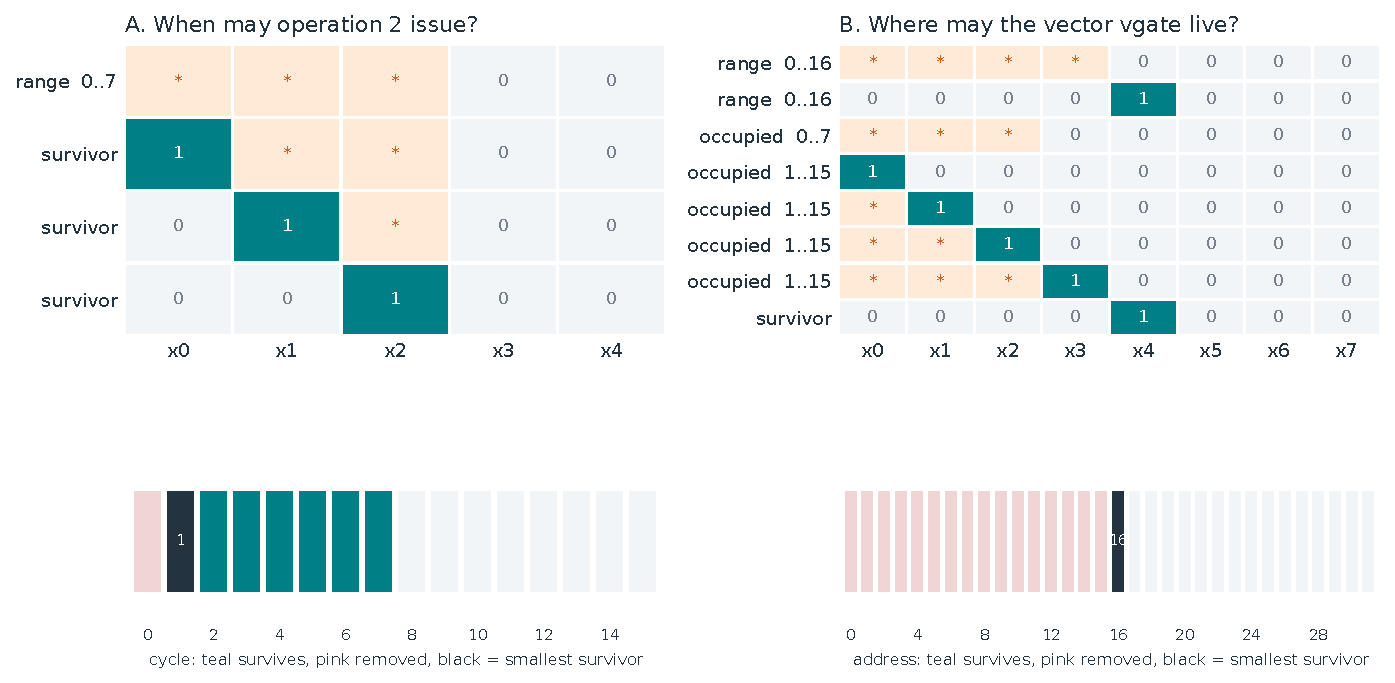
\includegraphics[width=\linewidth]{we_index_queries.pdf}
\caption{\textbf{Two queries of the first answer, as the code evaluates them on
\texttt{05\_mixed\_broadcast}.} Each row of the upper panels is a cube over the
coordinates $x_0,x_1,\dots$ (teal $1$, grey $0$, orange $*$ free). (A)~Operation~\V{weQTop} may
issue in cycles \V{weQTlo} to \V{weQThi}, one cube; cycle \V{weQTlo} is removed
because the load engine is already full there, which leaves \V{weQTsurv} cubes
whose smallest member, cycle \V{weQTchosen}, is chosen. (B)~The vector
\texttt{vgate} may start at any aligned address up to \V{weQAhi}; the blocks held
by the two vectors whose lifetimes overlap it are removed, and the smallest
surviving aligned address, \V{weQAchosen}, is chosen. The lower strips expand the
same sets for reading; the implementation never enumerates them. Every cover
shown is recorded from the real run and checked for exactness before rendering.}
\label{fig:index}
\end{figure}

\section{From the first answer to C1}\label{sec:c1}

The first answer never revisits a decision. Everything after it does, and it does
so by asking a sequence of exact questions, each of which is small enough to
answer completely. Figure~\ref{fig:pipeline} follows one epoch of this process
on the worked example.

\paragraph{Windows.} Reopening every decision at once is hopeless, and reopening
one at a time finds almost nothing, because useful changes move several
operations together. Following Shaw's large neighbourhood search~\cite{shaw1998},
C1 builds a catalogue of \emph{windows}: groups of related operations whose issue
cycles may move within a radius, with everything else held fixed. The catalogue
mixes the four-operation windows of the first version, the $k$ latest-issued
operations (which decide $C$), the $k$ operations around the memory peak (which
decide $S$), contiguous blocks of $k$, and the whole program when it is small.

\paragraph{Product caps.} For a window, the fixed decisions alone give lower
bounds $L_C$ and $L_S$ on any completion. A strict improvement needs
$C\,S\leq J_0-1$, hence $C\leq\lfloor (J_0-1)/L_S\rfloor$ and
$S\leq\lfloor (J_0-1)/L_C\rfloor$. Every strict improvement lies in this box, so
the domain may be cut to it without losing any; when a cap falls below its lower
bound the window is proved empty. This replaced the target rectangles of the
first version, which leave parts of the region below the hyperbola unexamined.

\paragraph{Certified propagation.} Inside the box, each reopened operation has an
ordered list of candidate cycles whose first entry is its current cycle.
Propagation removes values that cannot appear in any solution, and every removal
emits a \emph{certificate}: a tuple that anyone holding the program can check in
one line. A precedence certificate records that $v$ reads $u$ with lag $\ell$, so
that $v$ cannot issue before $\min D_u+\ell$ (\textsf{PL}) and $u$ cannot issue
after $\max D_v-\ell$ (\textsf{PU}); capacity certificates remove cycles whose
slots are all occupied (\textsf{EF}) or prove a branch impossible (\textsf{EO}).
This discipline of explained propagation is taken from lazy clause
generation~\cite{ohrimenko2009}; clause learning itself is not used.

\paragraph{Exact search and the controller.} What propagation cannot rule out,
a depth-first branch and bound decides, pruning a node when a lower bound on $J$
is no better than the best known. A controller keeps \V{resident} questions resident and
gives each a slice of at most \V{sliceMs}\,ms or \V{sliceNodes} nodes in turn. The first question to
find a strict improvement wins: its answer is validated by the challenge's own
checker, becomes the new incumbent, and a new epoch begins with a fresh catalogue.
This is the combinatorial approach to scheduling and allocation of Casta\~neda
Lozano and colleagues~\cite{castaneda2019}, applied to small neighbourhoods of one
incumbent rather than to a whole function.

\paragraph{The shared branch state.} In R0 each child node copies its parent's
domains and recomputes the whole fixed point, although it differs from the parent
by one decision. C1 keeps at each node an immutable branch state (its domains and
the facts derived from them) together with a change record of which domains lost
their extreme values or became single cycles, and each rule re-examines only the
constraints that the change can reach (Figure~\ref{fig:shared}). This is
incremental, event-driven propagation, a well-established idea in constraint
programming~\cite{schulte2008}, and we claim no novelty for it. The contribution
is narrower: an exact emulation of R0's sweep order, so that C1 emits the same
certificates in the same order, together with an empirical parity test of that
property.

\begin{figure}[htbp]\centering
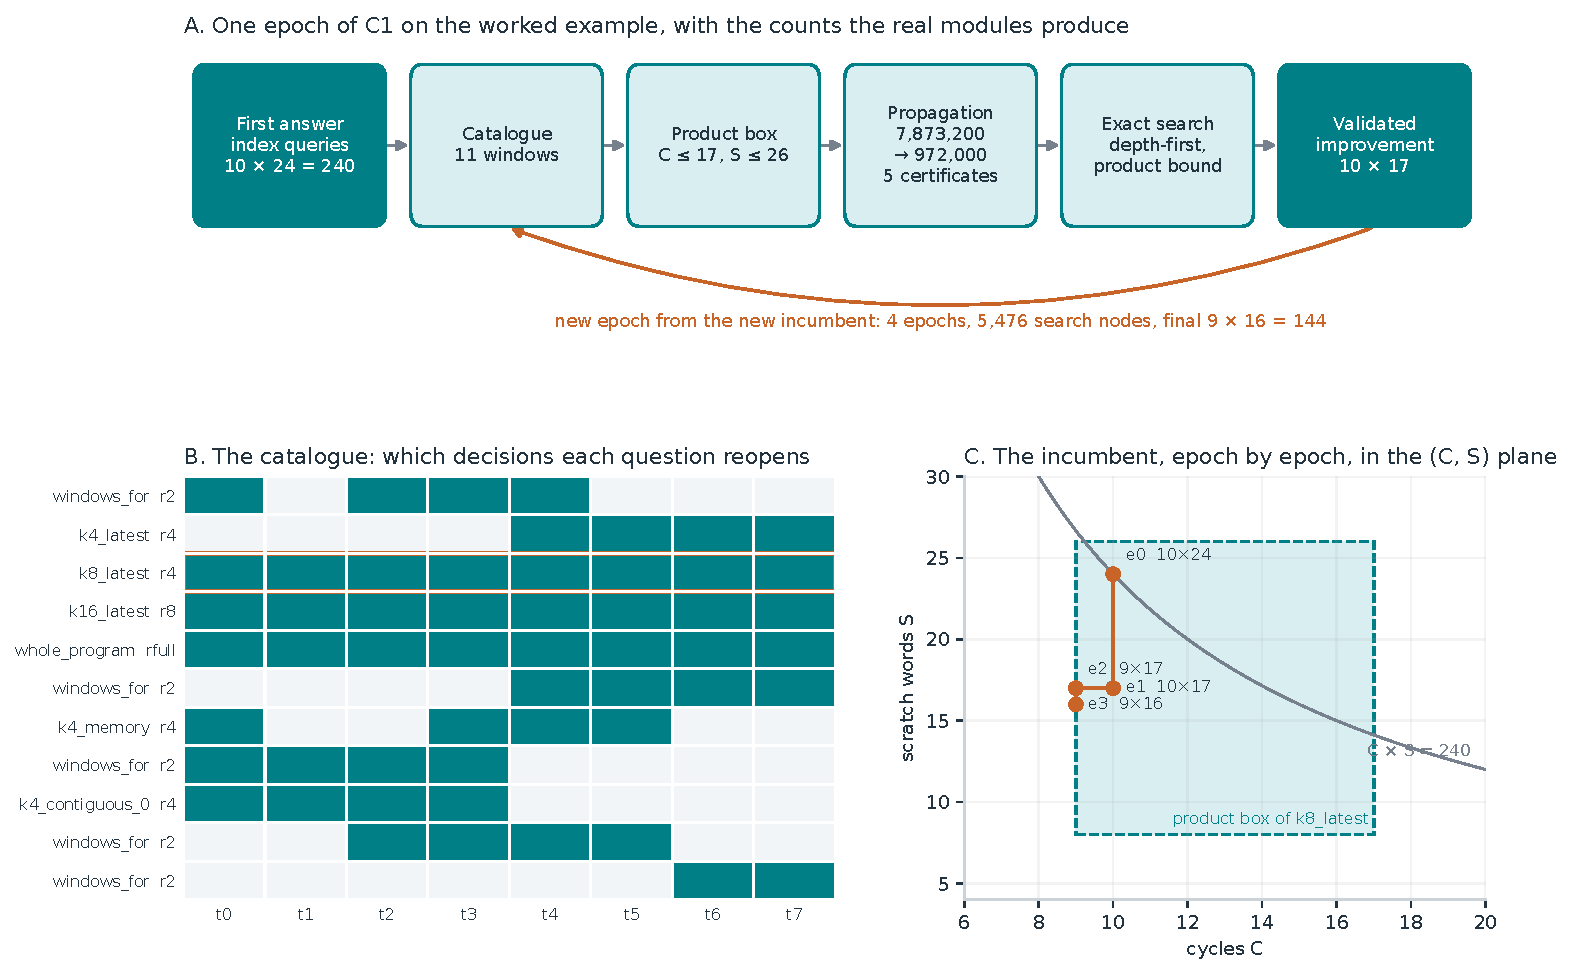
\includegraphics[width=\linewidth]{we_pipeline.pdf}
\caption{\textbf{C1 on the worked example.} (A)~One epoch as an operation
network, annotated with the counts the real modules produce: \V{weCatalogue}
windows; the product box of the \texttt{k8\_latest} window, $C\leq\V{weCapCcap}$ and
$S\leq\V{weCapScap}$; propagation that reduces the declared time combinations from
\V{weCombDeclared} to \V{weCombRoot} with \V{weRootCerts} certificates; and the
validated improvement. (B)~The catalogue: each row is one question and each
filled cell an operation it may move. (C)~The incumbent in the $(C,S)$ plane over
\V{weEpochs} epochs and \V{weNodes} search nodes at fixed work; the first
improvement lies inside the product box. All counts are checked before
rendering; they describe one program and are not evidence of average gain.}
\label{fig:pipeline}
\end{figure}

\begin{figure}[htbp]\centering
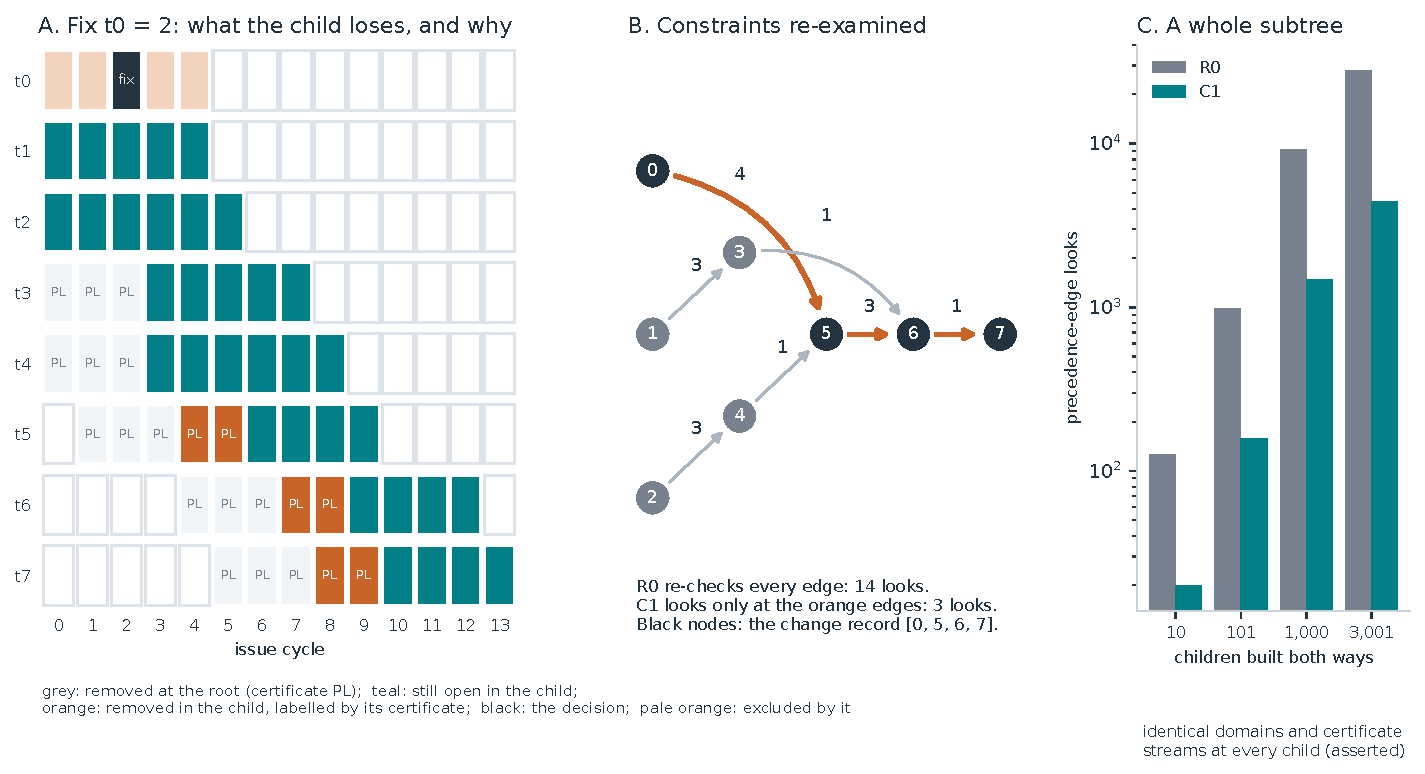
\includegraphics[width=\linewidth]{we_shared_state.pdf}
\caption{\textbf{One propagation step, and the shared branch state.} (A)~Fixing
operation~\V{weChildOp} at cycle~\V{weChildVal} in the \texttt{k8\_latest} question: grey cells were
removed at the root, orange cells are removed in the child and are labelled by the
certificate that removed them. (B)~The \V{weEdges} precedence constraints; for this child
R0 re-examines every one (\V{weLooksR} edge looks) while C1 re-examines only the
orange ones (\V{weLooksC} looks). (C)~Over a depth-first subtree of \V{weSubChildren}
children built both ways, R0 makes \V{weSubR} edge looks and C1 \V{weSubC}; the
domains and the \V{weSubCerts} certificates are identical at every child, which the
generator asserts. The same counts are printed by notebook~04, and the generator
checks that they agree.}
\label{fig:shared}
\end{figure}

\section{A worked example, method by method}\label{sec:worked}

We now run every method on one public program, \texttt{05\_mixed\_broadcast}
(Figure~\ref{fig:program}). It has \V{weOps} operations: three loads, two
\texttt{splat}s that copy a scalar into all lanes of a vector, a vector multiply,
a vector add and a store. Its trade-offs are visible at a glance: the vector load
is slow, two vectors must be alive at once, and the order in which they are
created decides how much scratch they need. Every number in this section describes
this one program and is illustrative; none of it is evidence of an average gain.

\begin{figure}[htbp]\centering
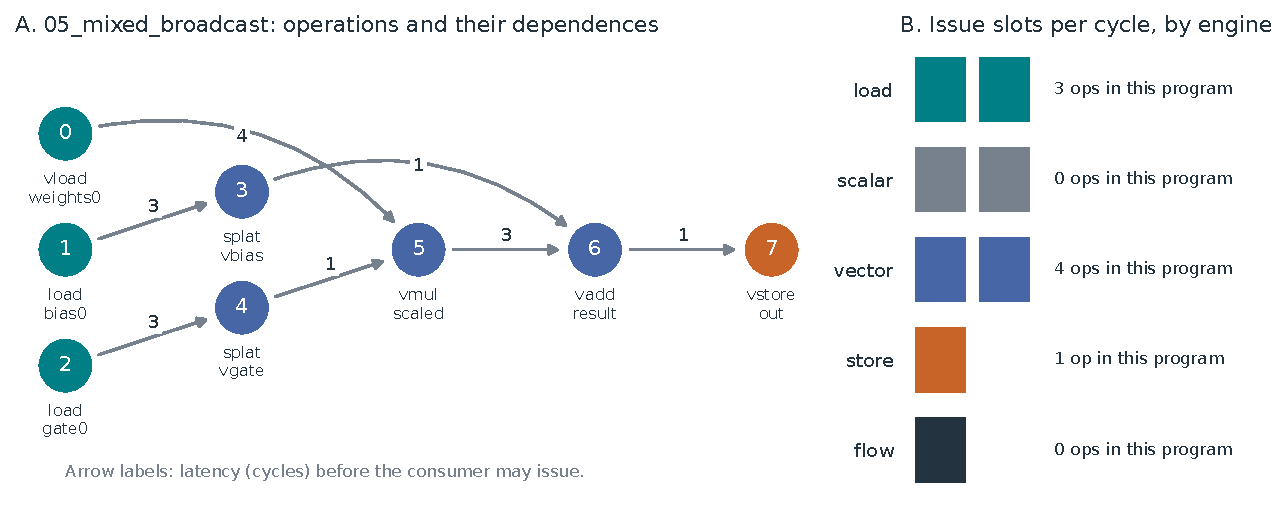
\includegraphics[width=\linewidth]{we_program.pdf}
\caption{\textbf{The worked example.} (A)~The dependence network of
\texttt{05\_mixed\_broadcast}; colour marks the engine and arrow labels the latency
that must elapse before the consumer may issue. (B)~The machine's issue slots per
cycle. The generator checks that every arrow's label equals its producer's
latency.}\label{fig:program}
\end{figure}

Figure~\ref{fig:methods} aligns the five methods' schedules and scratch layouts,
and Table~\ref{tab:worked} gives their metrics. The serial and starter compilers
follow a fixed rule and produce the same answer, \V{weSerialC}~cycles and
\V{weSerialS}~words. The classical compiler follows local priorities: it issues
the operations with the longest remaining path first and places each value at the
lowest free address, reaching \V{weClassicalC}~×~\V{weClassicalS}. It never
revisits a decision, and on this program its greedy choices happen to be good.

The original direct compiler states each choice as an exact query, so every cycle
and address it emits is a witness of a stated set: the smallest member of a cover.
Its answer, \V{weDirectphase1C}~×~\V{weDirectphase1S}, is \emph{worse} than the
classical one on both counts. The smallest-index rule places each vector as soon
as it can, which keeps two eight-word vectors alive together, and the first
version's four-operation windows cannot move enough operations at once to undo
this. This is the program on which the first version lost, and it is why the
later stages exist.

C1 starts from that same first answer and reopens it. Its first epoch, through the
\texttt{k8\_latest} window that releases all eight operations, keeps every cycle
and cuts the footprint to \V{weStepAS} words. The second, through the same window,
saves a cycle. The third, through an ordinary four-operation window that had
nothing to offer from the first answer, saves one more word, ending at
\V{weC1C}~×~\V{weC1S} (Figure~\ref{fig:pipeline}C). The large move opened the way
and a small one finished it. At fixed work R0 walks exactly the same path: the
search traces and certificate streams of the two compilers have identical hashes
on this program, as on every tested program. At a wall-clock allowance of \V{bA}\,s
the difference in speed becomes visible in the output: C1 reaches
\V{wePubC1Shortcycles}~×~\V{wePubC1Shortscratch} and R0
\V{wePubR0Shortcycles}~×~\V{wePubR0Shortscratch}. On the larger public program
\texttt{08\_vector\_reduction}, with \V{weScaleOps} operations, the same search
lowers $J$ from \V{weScaleFirstJ} to \V{weScaleFinalJ} within \V{weScaleNodes}
nodes.

\begin{figure}[htbp]\centering
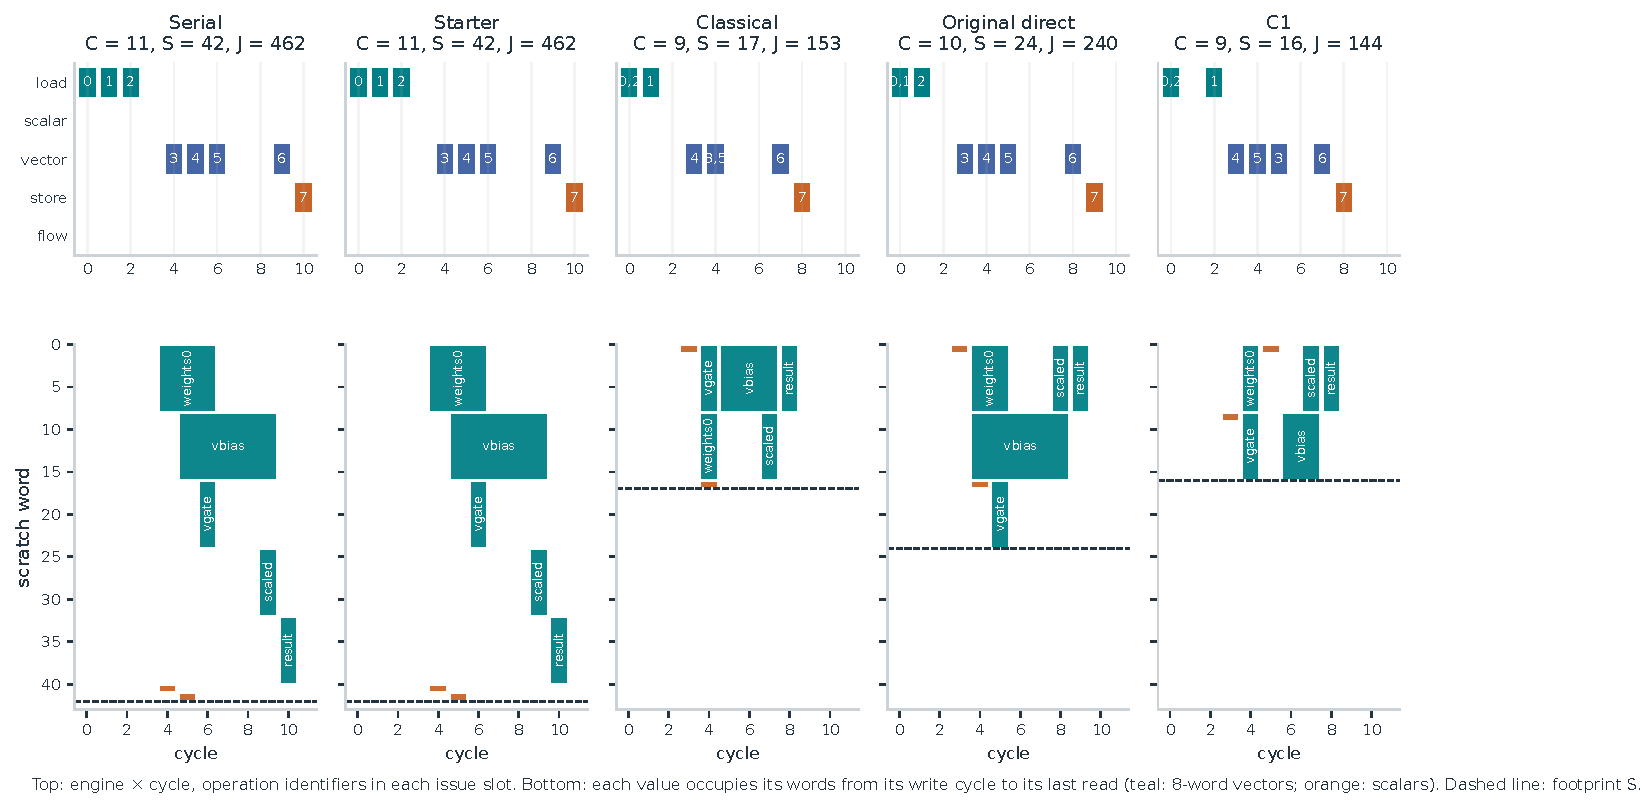
\includegraphics[width=\linewidth]{we_methods.pdf}
\caption{\textbf{Five methods, one program.} Top: the schedule as engine ×
cycle, with the identifiers of the operations issued in each slot. Bottom: the
scratch layout, each value occupying its words from its write cycle to its last
read; the dashed line is the footprint $S$. Every layout is produced by running
the method, validated by the challenge's checker on every test case, and checked
for capacity and for live overlaps before rendering.}\label{fig:methods}
\end{figure}

\begin{table}[htbp]\centering\scriptsize
\begin{tabularx}{\linewidth}{lrrr>{\raggedright\arraybackslash}p{36mm}>{\raggedright\arraybackslash}X}
\toprule
Method & $C$ & $S$ & $J$ & Compile call (frozen evidence) & Mechanism\\\midrule
\tableinput{generated/tab_worked.tex}
\bottomrule
\end{tabularx}
\caption{The worked example, one program. Compile times are medians from the
frozen measurement runs, never measured here: serial from the Phase~1
comparison, classical and original direct from the Phase~1 timing run (full mode),
C1 from the third-round public stage. They were recorded in different runs of one
machine and are shown for scale only. The starter compiler was never timed.}
\label{tab:worked}
\end{table}

The contrast is between kinds of reasoning, not between scores on one program.
The serial and starter compilers apply a fixed rule. The classical compiler
applies greedy local priorities and cannot undo a commitment. The direct method
expresses each choice as an exact statement about a set, so any answer can be
traced to the set it was drawn from. C1 then reopens related groups of decisions,
confines each question to the only region where a strict improvement can exist,
deletes impossible options with a local causal reason (``because $v$ reads $u$ with
lag $\ell$''), searches the rest exactly, and reuses at each node the facts its
parent derived.

\section{Evaluation design}\label{sec:design}

\paragraph{Populations.} All generated programs come from the same generator in
five families (scalar, vector, mixed, dependency and aliasing). The final round
developed and selected its mechanism on development seeds and confirmed it on a
fresh cohort of \V{tPrograms} programs, \V{tPerFamily} per family, seeds
\V{tSeedLo}--\V{tSeedHi}, generated only after C1 had been frozen by hash. None of
the cohort's program, file or compilation-input hashes occurs in any earlier result
file. Earlier rounds used their own fresh cohorts, which are never pooled.

\paragraph{Endpoints.} Two endpoints were registered before measurement. The cost
endpoint is the complete compile-call time at fixed work: the search is limited to
\V{tNodes} nodes on a logical clock that never advances, so both arms perform the
same search. The quality endpoint is $J$ at a real \V{bB}\,s allowance. Each program
was compiled \V{tReps} times by each arm in fresh processes. The estimator is the
equal-family geometric mean of per-program median ratios, with a paired bootstrap
over programs stratified by family (\V{tResamples} resamples, seed \V{tSeed},
percentiles \V{tPctLo} and \V{tPctHi}, a Bonferroni split across the two
endpoints). The gates were an upper bound of at most \V{tGateCost} for cost and at
most \V{tGateQual} for quality, with exact parity at fixed work.

\paragraph{Correctness.} Every compilation in every stage was validated by the
challenge's evaluator on every supplied case. Both standalone exports pass a
corpus of \V{tAccPrograms} programs and \V{tAccCases} cases. All
\V{tExportRows} command-line runs of the exports were re-validated by the review
with the challenge's own evaluator.

\paragraph{Review.} Codex, the designated lead reviewer, was unavailable for the
final round, and the author authorised Claude Code to complete the review. The
reviewer was therefore also the implementer, and the acceptance of C1 is a
self-review. It recomputed every endpoint with new standard-library code that
imports neither the reporter nor the auditor, re-validated the exports, repeated
the bootstrap under three further seeds (upper cost bounds \V{tAltSeedACostHi},
\V{tAltSeedBCostHi} and \V{tAltSeedCCostHi}), and probed for order effects, drift,
timer scope and heterogeneity. It also found two errors in the implementer's own
handoff, reported in Supplementary Section~\ref{S-sec:errata}. An independent
re-review would supersede it.

\section{Results}\label{sec:results}

\subsection{The final proposal against its predecessor}
C1 met both gates with a wide margin (Table~\ref{tab:c1}). At fixed work the two
compilers made the same decisions: \V{tParityPairs} of \V{tParityPairs} paired runs
had identical search traces, incumbents, statuses and certificate streams
(\V{tTraces} distinct traces over \V{tPrograms} programs; a median of
\V{tCertMedian} certificates per run). Of those pairs, \V{tSubstantive} involve real
search, because \V{tZeroNode} programs need no search node at all. Parity holds on
every tested input; it is not a proof for all programs. At that equal work C1's
complete compile call took \V{tCost} of R0's time, with \V{lvThree}\% interval
\ci{\V{tCostLo}}{\V{tCostHi}}; at the \V{bB}\,s allowance its $J$ ratio was \V{tQual},
with interval \ci{\V{tQualLo}}{\V{tQualHi}}.

\begin{table}[htbp]\centering\small
\begin{tabular}{lrrl}\toprule
Endpoint (C1 / R0, \V{tPrograms} fresh programs) & Estimate & \V{lvThree}\% interval & Gate\\\midrule
Compile call at fixed work (\V{tNodes} nodes) & \V{tCostFour} & \ci{\V{tCostLoFour}}{\V{tCostHiFour}} & $\leq\V{tGateCost}$\\
$J$ at \V{bB}\,s & \V{tQualFour} & \ci{\V{tQualLoFour}}{\V{tQualHiFour}} & $\leq\V{tGateQual}$\\
Parity at fixed work & \multicolumn{2}{l}{\V{tParityPairs} / \V{tParityPairs} pairs identical} & exact\\
\bottomrule\end{tabular}
\caption{The registered endpoints of the final round, with the estimator and
bootstrap described in Section~\ref{sec:design}. Both are ratios C1/R0; lower is
better. The independent recomputation reproduced both estimates exactly.}\label{tab:c1}
\end{table}

The descriptive probes support the same reading. Adding the solver-module import
time gives a cost ratio of \V{tImport}, and whole-process time including
interpreter start gives \V{tProcess}; the shared base compile and validation lie
inside both arms and pull the ratio towards one. Splitting pairs by which arm ran
first gives \V{tOrderR0} (\V{tOrderR0Pairs} pairs, R0 first) and \V{tOrderC1}
(\V{tOrderC1Pairs} pairs, C1 first), and the ratio shows no trend across time
quartiles (\V{tDriftA}, \V{tDriftB}, \V{tDriftC}, \V{tDriftD}). Per program the
ratio ranges from \V{tPPmin} to \V{tPPmax} (median \V{tPPmedian}), and C1 is slower
on \V{tPPslower} of \V{tPrograms} programs (Figure~\ref{fig:perprog}). The saving
grows with the size of the search, as a mechanism that reuses parent facts at every
node predicts: \V{tTerA} on the smallest third of programs by search size,
\V{tTerB} on the middle third and \V{tTerC} on the largest. In wall-clock mode C1's
compile call is never longer (geometric ratios \V{tWallTimeA}, \V{tWallTimeB} and
\V{tWallTimeC} at allowances of \V{bA}, \V{bB} and \V{bC}\,s), so its quality is not bought
with extra time. At the \V{bB}\,s allowance C1 is better on \V{tWTLBW}, equal on
\V{tWTLBT} and worse on \V{tWTLBL} of the paired runs; per program, \V{tProgBetter}
are better, \V{tProgEqual} equal and \V{tProgWorse} worse.

\begin{figure}[htbp]\centering
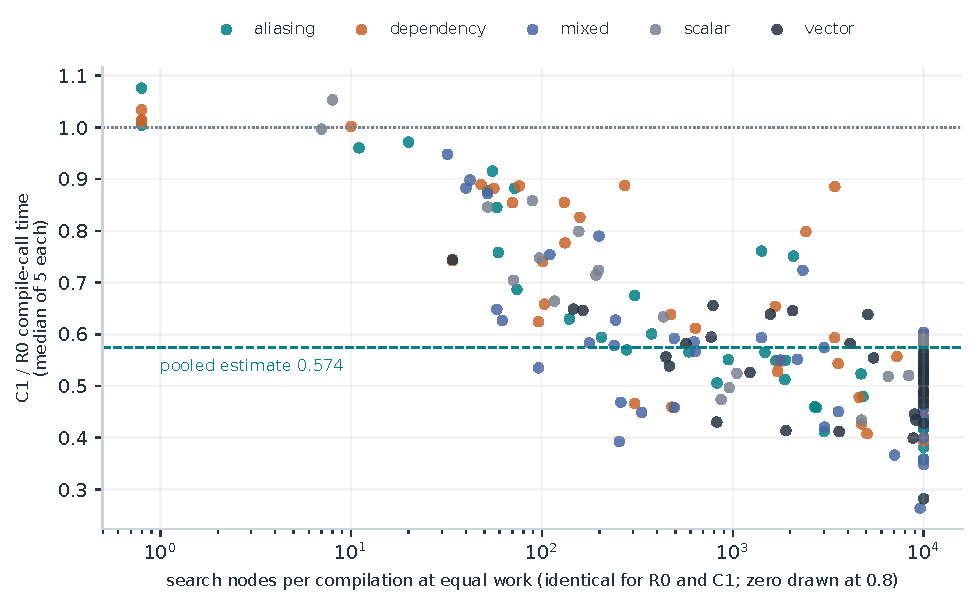
\includegraphics[width=.9\linewidth]{results_per_program.pdf}
\caption{\textbf{C1/R0 compile-call time at equal work, one point per fresh
program}, against the number of search nodes, which is identical for both arms.
The dashed line is the confirmatory estimate. Ratios near one on tiny searches
reflect fixed costs that both arms share; the saving grows with the search. The
generator checks the minimum, maximum, median and number of programs above one
against the independent recomputation.}\label{fig:perprog}
\end{figure}

This is an engineering property of one Python implementation, measured on one
local machine at equal search work. It is not a result about computational
complexity, not a private-grader result, and not a comparison with the compile
time of the classical compiler. Memory is a cost: the peak traced allocation of C1
relative to R0 had a median of \V{tMemMed} and a maximum of \V{tMemMax}, measured
on \V{tMemPrograms} development programs only; no memory measurement exists for the
confirmation cohort.

\subsection{Speed changes the path}\label{sec:q1}
Decision parity holds at equal work. Under a real clock it does not hold program by
program, and the reason is instructive. The controller gives each resident
question a slice of \V{sliceMs}\,ms or \V{sliceNodes} nodes, and the first strict improvement ends the
epoch. C1 expands more nodes per slice, so a different question can be the first
to improve, and from there the two searches follow different paths. At a \V{bC}\,s
allowance C1 is worse than R0 on \V{tLossRuns} of the paired runs, spread over
\V{tLossPrograms} programs; it is deterministic across repetitions on those
programs, and \V{tLossNoUnknown} of the losses involve no unresolved question on
either side. On program \V{tQoneSeed} both start from the same first answer,
\V{weQone980183C}~×~\V{weQone980183S}; R0 ends at
\V{tSeed980183R0cycles}~×~\V{tSeed980183R0scratch}~$=\V{tSeed980183R0J}$ and C1 at
\V{tSeed980183C1cycles}~×~\V{tSeed980183C1scratch}~$=\V{tSeed980183C1J}$, in all \V{tReps}
repetitions (Figure~\ref{fig:q1}). The quality claim is therefore distributional,
and it is stated as ``decision parity at equal work'', never as a claim that the two compilers
decide alike under a wall budget, nor that C1 is never worse.

This is not a defect of C1; it is a property of anytime first-improvement local
search on a rugged landscape. A faster search reaches a different basin, and a
different basin can be worse. Being faster does not imply being better.

\begin{figure}[htbp]\centering
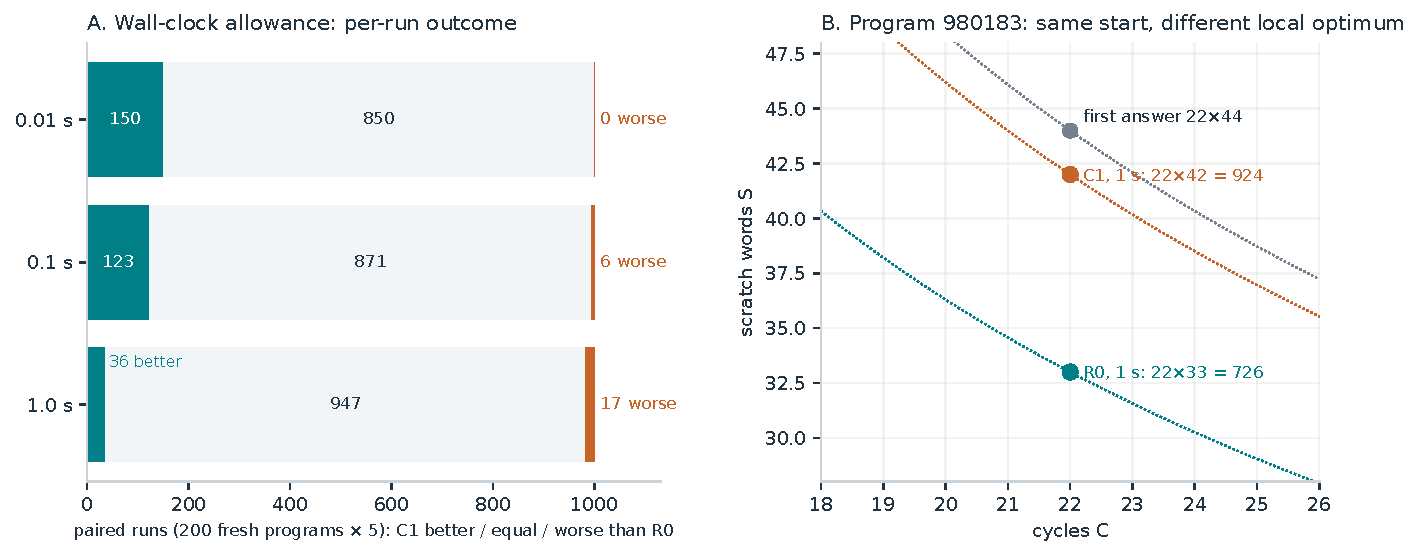
\includegraphics[width=\linewidth]{results_q1.pdf}
\caption{\textbf{Quality is not monotone in speed.} (A)~Paired runs at three
wall-clock allowances (\V{tPrograms} fresh programs, \V{tReps} repetitions): C1
better, equal or worse than R0. (B)~Program \V{tQoneSeed} at \V{bC}\,s: the same first answer,
and two different local optima that each arm reached in every repetition; dotted
curves are lines of constant $J$. The generator checks that the generated program
is byte-identical to the one the frozen rows measured.}\label{fig:q1}
\end{figure}

\subsection{The whole programme against the benchmarks}
Table~\ref{tab:public} gives the public score of every method, and
Table~\ref{tab:perprogram} the per-program metrics of the external benchmarks, our
first version and C1. The public programs were visible throughout development,
so these are exact results on eight fixed programs, not estimates for a
population. On them the programme moved from \V{pOneScore} (first version) to
\V{tPubSixC1B} (C1 at \V{bB}\,s), against \V{rTwoPubClassical} for the classical
compiler.

\begin{table}[htbp]\centering\small
\begin{tabular}{llll}\toprule
Method & Role & Allowance & Public score\\\midrule
\tableinput{generated/tab_public.tex}
\bottomrule\end{tabular}
\caption{Score (Equation~\ref{eq:score}) on the \V{mPublic} public programs,
relative to serial; higher is better. Every value was identical in every
repetition of its run. Scores from different rounds are exact on the same
programs, so they may be compared, but they are not population estimates; the
round-two row for \texttt{cap512\_wider} shows why (Section~\ref{sec:negative}).}
\label{tab:public}
\end{table}

\begin{table}[htbp]\centering\small
\begin{tabular}{lllllrrrr}\toprule
& \multicolumn{4}{c}{$C\times S$} & \multicolumn{4}{c}{$J$}\\
\cmidrule(lr){2-5}\cmidrule(lr){6-9}
Program & Serial & Classical & Direct & C1 & Serial & Classical & Direct & C1\\\midrule
\tableinput{generated/tab_perprogram.tex}
\bottomrule\end{tabular}
\caption{Per-program metrics on the public programs. Direct is the original
direct compiler (its bootstrap and full modes give identical public metrics); C1 is
at the \V{bB}\,s allowance, where R0 gives the same metrics. Bold marks the lowest
$J$ in each row. Values are constant across all repetitions.}\label{tab:perprogram}
\end{table}

On fresh populations the picture is more nuanced, and every measured pair appears
in Figure~\ref{fig:forest} and Table~\ref{tab:pairs} with its own comparator. The
closest measured comparison of our search with the classical compiler is from
round one: at \V{bB}\,s the A4 search found \V{rOneClRed}\% lower geometric $J$ than
classical (\V{lvOne}\% interval \V{rOneClLo}\% to \V{rOneClHi}\%) on \V{tPrograms} fresh
programs, winning on \V{rOneClwins}, tying on \V{rOneClties} and \emph{losing on
\V{rOneCllosses}}, at \V{rOneClTime} times classical's compile time. In round two
the depth-first variant that became R0 was descriptively \V{rTwoDfsClRed}\% better
than classical on another fresh cohort (\V{rTwoDfsClW} wins, \V{rTwoDfsClT} ties,
\V{rTwoDfsClL} losses, unadjusted). C1 itself was never measured against classical
on a fresh cohort; we do not chain C1/R0 onto these ratios.

\begin{figure}[htbp]\centering
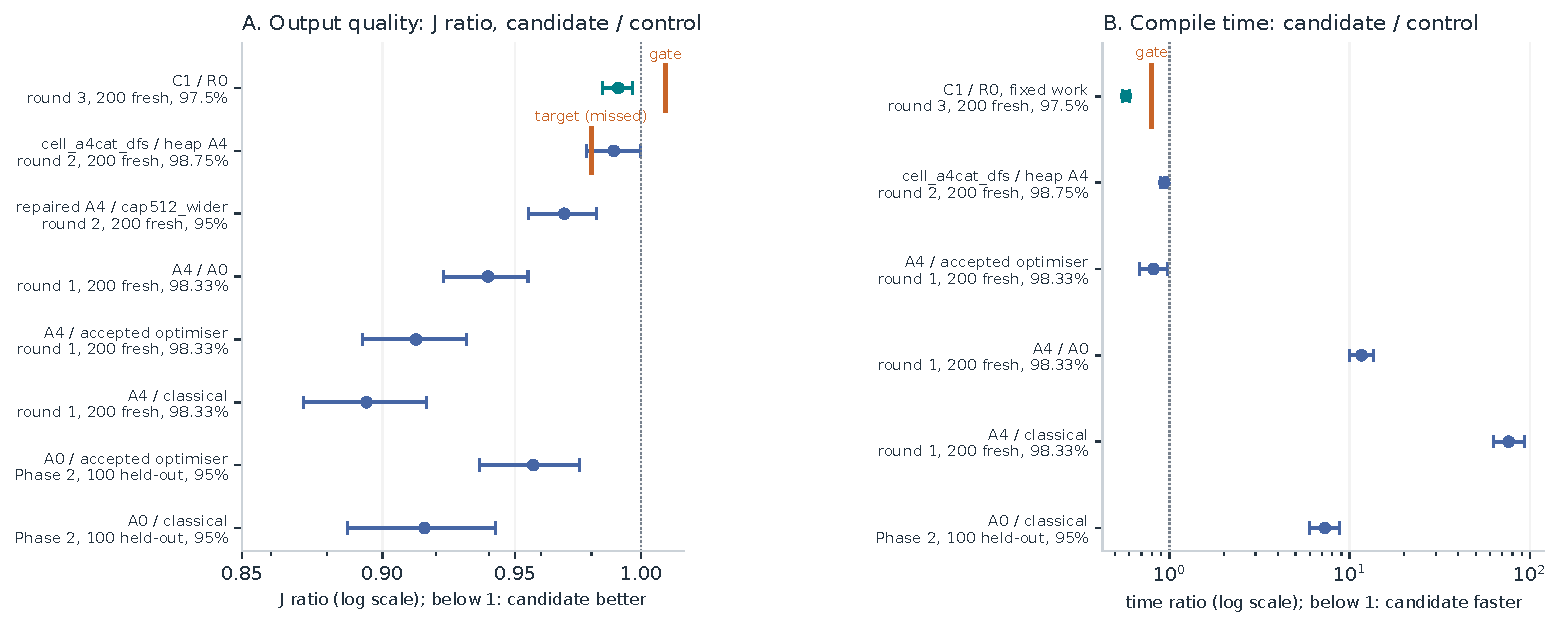
\includegraphics[width=\linewidth]{results_forest.pdf}
\caption{\textbf{Every measured pair, each against its own control.} (A)~Output
quality as the geometric $J$ ratio of candidate to control; (B)~compile time as the
geometric ratio of candidate to control. Each row names its round, population and
interval level. Orange bars are registered gates or targets: C1's gates were met;
the round-two practical target of \V{rTwoQRoute} was missed (TARGET\_NOT\_REACHED).
Rows are never combined across rounds.}\label{fig:forest}
\end{figure}

\begin{table}[htbp]\centering\scriptsize
\begin{tabularx}{\linewidth}{>{\raggedright\arraybackslash}p{36mm}>{\raggedright\arraybackslash}X>{\raggedright\arraybackslash}p{33mm}rr}
\toprule
Pair (candidate / control) & Population, allowance, interval & Quality & W / T / L & Time ratio\\\midrule
C1 / R0 & round 3, \V{tPrograms} fresh, \V{bB}\,s; \V{lvThree}\% & $J$ ratio \V{tQual} \ci{\V{tQualLo}}{\V{tQualHi}} & \V{tWTLBW} / \V{tWTLBT} / \V{tWTLBL} & \V{tCost}$^{a}$\\
\texttt{cell\_a4cat\_dfs} / heap A4 & round 2, \V{tPrograms} fresh, \V{bB}\,s; \V{lvTwo}\% & $J$ ratio \V{rTwoDfsHJ} \ci{\V{rTwoDfsHLo}}{\V{rTwoDfsHHi}} & \V{rTwoDfsHnW} / \V{rTwoDfsHnT} / \V{rTwoDfsHnL} & \V{rTwoDfsHT}\\
\texttt{cell\_a4cat\_dfs} / \texttt{cap512\_wider} & round 2, \V{tPrograms} fresh, \V{bB}\,s; \V{lvTwo}\% & $J$ ratio \V{rTwoDfsEJ} \ci{\V{rTwoDfsELo}}{\V{rTwoDfsEHi}} & \V{rTwoDfsEnW} / \V{rTwoDfsEnT} / \V{rTwoDfsEnL} & \V{rTwoDfsET}\\
repaired A4 / \texttt{cap512\_wider} & round 2, \V{tPrograms} fresh, \V{bB}\,s; \V{lvStd}\% & $J$ ratio \V{rTwoJ}; mean log \V{rTwoLog} \ci{\V{rTwoLo}}{\V{rTwoHi}} & \V{rTwoWTLW} / \V{rTwoWTLT} / \V{rTwoWTLL} & \V{rTwoTime}\\
A4 / A0 & round 1, \V{tPrograms} fresh, \V{bB}\,s; \V{lvOne}\% & $J$ \V{rOneAzeroRed}\% lower \ci{\V{rOneAzeroLo}}{\V{rOneAzeroHi}}\% & \V{rOneAzerowins} / \V{rOneAzeroties} / \V{rOneAzerolosses} & \V{rOneAzeroTime}\\
A4 / accepted optimiser & round 1, \V{tPrograms} fresh, \V{bB}\,s; \V{lvOne}\% & $J$ \V{rOneAccRed}\% lower \ci{\V{rOneAccLo}}{\V{rOneAccHi}}\% & \V{rOneAccwins} / \V{rOneAccties} / \V{rOneAcclosses} & \V{rOneAccTimeThree}\\
A4 / classical & round 1, \V{tPrograms} fresh, \V{bB}\,s; \V{lvOne}\% & $J$ \V{rOneClRed}\% lower \ci{\V{rOneClLo}}{\V{rOneClHi}}\% & \V{rOneClwins} / \V{rOneClties} / \V{rOneCllosses} & \V{rOneClTime}\\
A0 / accepted optimiser & Phase 2, \V{aZeroAccN} held-out, \V{bB}\,s; \V{lvStd}\% & mean log \V{aZeroAccLog} \ci{\V{aZeroAccLo}}{\V{aZeroAccHi}} & \V{aZeroAccwins} / \V{aZeroAccties} / \V{aZeroAcclosses} & \V{aZeroAccTime}$^{b}$\\
A0 / classical & Phase 2, \V{aZeroClN} held-out, \V{bB}\,s; \V{lvStd}\% & mean log \V{aZeroClLog} \ci{\V{aZeroClLo}}{\V{aZeroClHi}} & \V{aZeroClwins} / \V{aZeroClties} / \V{aZeroCllosses} & \V{aZeroClTime}\\
Original direct / classical & Phase 1, \V{pOneExtraN} generated, default & score geomeans \V{pOneExtraFull} vs \V{pOneExtraCl} & \multicolumn{1}{c}{--} & \V{pOneSlowFull}\\
\bottomrule
\end{tabularx}
\caption{Every measured pair. Quality is reported in the statistic its protocol
registered; ``mean log'' is the mean paired $\log(J_{\text{control}}/J_{\text{candidate}})$,
positive when the candidate is better. W/T/L counts programs, except for C1/R0,
where it counts paired runs. Time ratios are geometric means of per-program median
compile times, candidate over control. $^{a}$At fixed work. $^{b}$A0 stops early, so
it finishes long before its allowance. No row may be multiplied by another.}
\label{tab:pairs}
\end{table}

\subsection{What the gains cost}
The method is slower to compile than the classical compiler, by a wide margin. In
round one, A4 took \V{rOneClTime} times classical's compile time (\V{lvOne}\% interval
\V{rOneClTimeLo} to \V{rOneClTimeHi}) and \V{rOneAzeroTime} times A0's. The first
version, in its full mode, took \V{pOneSlowFull} times classical's time, and even A0,
which stops early, took \V{aZeroClTime} times. C1 recovers part of the cost of its
own search (Table~\ref{tab:c1}), but nothing we measured suggests that it
approaches classical compile time, and we make no such claim. The quality gains
are also not uniform: A4 lost to classical on \V{rOneCllosses} of \V{tPrograms}
fresh programs, the first version was worse than classical on
\texttt{mixed\_broadcast} (Table~\ref{tab:perprogram}), and on generated programs
the first version's full mode was only marginally above classical (score geometric
means \V{pOneExtraFull} against \V{pOneExtraCl}). What the method offers is a
trade: better output on average, a reason for every deletion, and a search that can
be reopened, in exchange for compile time.

\section{What did not work}\label{sec:negative}

The negative results are part of the evidence, and each keeps its own comparator.
\begin{itemize}
\item \emph{The ladder.} Removing the query cap (A1) gained \V{ladOneQ} in mean log
$J$ over A0; product domains (A2) and certified propagation (A3) gained nothing in
quality (\V{ladTwoQ} and \V{ladThreeQ}), although each made compilation cheaper
(\V{ladTwoT} and \V{ladThreeT} times the previous step). Only the multiscale
catalogue (A4) moved quality, by \V{ladFourQ}, at \V{ladFourT} times A3's compile
time (Supplementary Section~\ref{S-sec:ladder}).
\item \emph{Catalogue, not traversal.} A two-by-two factorial on \V{facPrograms}
development programs attributed A4's gain to its catalogue ($\V{facCat}$ in log $J$,
\V{lvStd}\% interval \ci{\V{facCatLo}}{\V{facCatHi}}). The discrepancy-ordered traversal
of Harvey and Ginsberg~\cite{harvey1995} made no measurable difference
(\ci{\V{facTravLo}}{\V{facTravHi}}), and neither did the interaction.
\item \emph{A reversal between the public suite and the population.} On fresh
programs repaired A4 beat the earlier \texttt{cap512\_wider} optimiser (mean log
$J$ \V{rTwoLog}, \V{lvStd}\% interval \ci{\V{rTwoLo}}{\V{rTwoHi}}, with \V{rTwoWTLL} programs
worse), while on the public suite the order reversed, \V{rTwoPubCap} against
\V{rTwoPubHeap}. Neither result overrides the other; they answer different
questions.
\item \emph{A missed target.} The round-two candidate \texttt{cell\_a4cat\_dfs} was
better than A4 (J ratio \V{rTwoDfsHJ}) but missed both registered routes to a
``better'' claim (an upper $J$ bound of \V{rTwoQRoute}, or a compile-time upper bound
of \V{rTwoERoute} at no loss): TARGET\_NOT\_REACHED.
\item \emph{Two engineering attempts that stopped.} A worklist fixed point saved
\V{rTwoWorklist}\% of compile time against a gate of \V{rTwoWorklistGate}\%, and a
filter on the capacity rule was predicted to reach only \V{effPred} of the fixed-work
time against a gate of \V{tGateCost}: NO\_JUSTIFIED\_OPTIMIZATION.
\item \emph{The original registration of the shared branch state.} Its cost model
gave \V{tMReg} and stopped the round; the review found that one term was measured
over a narrower scope than the work it was meant to subtract. The correction is
post hoc and is reported as a forecast (\V{tMCons}), not as a measurement.
\item \emph{Learning.} A depth-three schema tree~\cite{breiman1984}, used in the
spirit of learned guidance for exact search~\cite{gasse2019}, lost to plain Hamming
order on all \V{lrnHamNeg} of \V{lrnFixtures} fixtures, and in \V{lrnEcoPrograms}
real compilations not one query collected the observations the learner needed
(\V{lrnEcoZero} of \V{lrnEcoPrograms}). Round one's learning hypothesis had failed by
design: none of its \V{rOneLearnOf} fixtures contained a test solution better than
the training minimum. The per-query learner is retired for this architecture.
\item \emph{Structural encoding.} The feasibility campaign behind A0 did not meet
its coverage gate and was recorded as inconclusive (Supplementary
Section~\ref{S-sec:feasibility}).
\end{itemize}

\section{Why a different way of computing}\label{sec:why}

The framing in this section is motivation and interpretation. The evidence is the
set of measured gains, costs and intervals above, and nothing said here adds to
it.

\paragraph{A lineage in work in progress.} The index-set method grows out of the
author's research on algorithmic information dynamics and the programmability of
integrated systems~\cite{hernandez2019aid,hernandez2021aid}, which in turn builds
on Zenil and collaborators' algorithmic information calculus and causal
deconvolution~\cite{zenil2017causality,zenil2019calculus,zenil2019deconvolution}.
Its broader form, index deconvolution, gives an exact finite representation of what
a system can do, as sets written in index form, from which behaviour can be
recovered, queried and explained. That method remains in development, and this
paper neither describes nor depends on its construction. What the compiler uses is
the narrower idea that a family of decisions can be stated exactly as a set of
indices and queried without enumeration. It is a specialisation of these ideas to
exact finite descriptions, and it is distinct from a computation of Kolmogorov
complexity itself.

\paragraph{Algorithmic information.} A cube is two integers that stand for a set
of any size, and a cover is a short exact description of which choices are legal.
The search asks, in effect, for the shortest exact statement of the region where a
better answer can lie, which is the program-length view of information of
Kolmogorov and Chaitin~\cite{kolmogorov1965,chaitin1966,li2019}. We compute no
Kolmogorov complexity and no estimate of it; the link is conceptual and
representational, not a measured quantity, and the parity bound of Supplementary
Section~\ref{S-sec:parity} shows that the representation compresses only what is
structured. The interest in simple exact rules that yield rich behaviour is
consonant with Wolfram's Principle of Computational Equivalence~\cite{wolfram2002,
wolfram2002pce}, which we use as motivation and not as a theorem about compilers.

\paragraph{Causality.} Every deletion of an option carries a certificate that
states a local reason and can be replayed by anyone holding the program. Reopening
a window and solving it again is an intervention on the schedule that holds the
rest fixed, in the sense of the interventional calculus of the cited
work~\cite{zenil2019calculus}. The result is a compiler whose every decision can be
audited: why a cycle was not used, which constraint forced a value to move, and
which question produced an improvement. A trained policy that emits a schedule does
not, by itself, offer this.

\paragraph{Complexity.} The problem is combinatorial and its landscape is rugged.
Large neighbourhoods of related decisions succeeded where local moves did not,
which is the lesson of large neighbourhood search~\cite{shaw1998}, and speed
changed the trajectory of the search (Section~\ref{sec:q1}), which is a hallmark of
path dependence in complex search. Both findings are measured; their
interpretation as features of a rugged landscape is ours.

\section{Limitations}\label{sec:limits}

The final mechanism was developed and selected on development programs, its
kernel draft preceded its specification, and its cost model was corrected after the
outcome; only the fresh confirmation is inferential. All measurements come from
one local machine and one Python implementation, and the speed-up is an
engineering property of that implementation, not an asymptotic result. The
public programs were visible throughout development, and there is no
private-grader result. Memory was measured on development programs only. All
generated programs come from one generator, so no claim transfers to real
compiler workloads without further evidence. Parity at equal work is established on
the tested inputs, not proved. The acceptance of C1 was a self-review. Finally, the
challenge asks that the exercise and its solution not be shared publicly; this
manuscript is prepared to publication standard but is kept local, and any release
requires that restriction to be resolved.

\section{Conclusion}\label{sec:conclusion}

We set out to answer the Luminal challenge and to test whether a different way of
computing is worth pursuing. The answer to the first is a compiler that is correct
on every supplied case, that scores \V{tPubSixC1B} on the public programs against
\V{rTwoPubClassical} for a classical list scheduler, and whose final stage runs the
same search in \V{tCost} of its predecessor's time at equal work without losing
quality at a fixed allowance. The answer to the second is more guarded and, we
think, more interesting. Stating every decision as an exact query over index sets
gave a compiler that can explain each of its choices, reopen any group of them, and
prove when a question has no better answer; the gains it earned came from asking
larger and better-shaped questions, and its costs are real and measured. As
compilation moves towards accelerators that expose every decision and towards
search and learning at scale, a representation that is exact, compact and
auditable is, on this evidence, worth developing further.

\section*{Code, data and assistance}
All figures and tables are regenerated from frozen evidence by the paper's build;
the worked example is produced by running the compilers themselves, and every
number cited is recorded, with its source file and field, in the claim ledger of
Supplementary Section~\ref{S-sec:ledger}. Claude Code assisted with implementation,
the final review and the preparation of this manuscript; Codex reviewed the earlier
rounds. The author is responsible for the claims and their interpretation.

\begin{thebibliography}{99}\raggedright\small
\bibitem{luminal} Luminal. \emph{Compiler challenge}, pinned source revision
573b8a85f4bdb8c3d8ba9f180d5f98dac875c902.
\url{https://github.com/luminal-ai/interview/tree/573b8a85f4bdb8c3d8ba9f180d5f98dac875c902}.
\bibitem{hernandez2019aid} A. Hernández-Espinosa, H. Zenil, N. A. Kiani and
J. Tegnér, \emph{Estimations of Integrated Information Based on Algorithmic
Complexity and Dynamic Querying}, arXiv:1904.10393 [q-bio.NC] (2019).
\url{https://arxiv.org/abs/1904.10393}.
\bibitem{hernandez2021aid} A. Hernández-Espinosa, H. Zenil, N. A. Kiani and
J. Tegnér, ``Estimations of Integrated Information Based on Algorithmic
Complexity and Dynamic Querying,'' in \emph{Handbook of Unconventional
Computing}, Vol. 1: Theory, ed. A. Adamatzky (World Scientific, 2021), Chap. 5,
pp. 171--220.\ \url{https://doi.org/10.1142/9789811235726_0005}.
\bibitem{kolmogorov1965} A. N. Kolmogorov, \emph{Three approaches to the
definition of the concept of quantity of information}, \emph{Problems of
Information Transmission} 1(1), 3--11 (1965); English reprint,
\emph{Three Approaches to the Quantitative Definition of Information},
\emph{International Journal of Computer Mathematics} 2(1--4), 157--168
(1968).\\ \url{https://doi.org/10.1080/00207166808803030}.
\bibitem{chaitin1966} G. J. Chaitin, \emph{On the length of programs for
computing finite binary sequences}, \emph{Journal of the ACM} 13(4),
547--569 (1966).\\ \url{https://doi.org/10.1145/321356.321363}.
\bibitem{li2019} M. Li and P. M. B. Vitányi, \emph{An Introduction to
Kolmogorov Complexity and Its Applications}, 4th ed., Texts in Computer
Science (Springer, Cham, 2019).\\ \url{https://doi.org/10.1007/978-3-030-11298-1}.
\bibitem{wolfram2002} S. Wolfram, \emph{A New Kind of Science}, Chap. 12
(Wolfram Media, Champaign, IL, 2002).\\
\url{https://www.wolframscience.com/nks/}.
\bibitem{wolfram2002pce} S. Wolfram, ``Notes for Chapter 12: The Principle
of Computational Equivalence,'' in \emph{A New Kind of Science Online}
(2002).\ \url{https://www.wolframscience.com/reference/notes/1128c/}.
\bibitem{zenil2017causality} H. Zenil, A. Schmidt and J. Tegnér,
\emph{Causality, Information, and Biological Computation: An Algorithmic
Software Approach to Life, Disease, and the Immune System}, in \emph{From
Matter to Life: Information and Causality}, eds. S. I. Walker, P. C. W. Davies
and G. F. R. Ellis (Cambridge University Press, 2017), pp. 244--280.
\url{https://doi.org/10.1017/9781316584200.011}.
\bibitem{zenil2019calculus} H. Zenil, N. A. Kiani, F. Marabita, Y. Deng,
S. Elias, A. Schmidt, G. Ball and J. Tegnér, \emph{An Algorithmic Information
Calculus for Causal Discovery and Reprogramming Systems}, \emph{iScience}
19, 1160--1172 (2019).\\ \url{https://doi.org/10.1016/j.isci.2019.07.043}.
\bibitem{zenil2019deconvolution} H. Zenil, N. A. Kiani, A. A. Zea and
J. Tegnér, \emph{Causal deconvolution by algorithmic generative models},
\emph{Nature Machine Intelligence} 1, 58--66 (2019).
\url{https://doi.org/10.1038/s42256-018-0005-0}.
\bibitem{shaw1998} P. Shaw, \emph{Using Constraint Programming and Local Search
Methods to Solve Vehicle Routing Problems}, in \emph{Principles and Practice of
Constraint Programming -- CP98}, eds. M. Maher and J.-F. Puget, LNCS 1520
(Springer, 1998), pp. 417--431. \url{https://doi.org/10.1007/3-540-49481-2_30}.
\bibitem{harvey1995} W. D. Harvey and M. L. Ginsberg, \emph{Limited Discrepancy
Search}, in \emph{Proceedings of the 14th International Joint Conference on
Artificial Intelligence (IJCAI-95)}, Vol. 1, pp. 607--613 (1995).
\url{https://www.ijcai.org/Proceedings/95-1/Papers/080.pdf}.
\bibitem{castaneda2019} R. Castañeda Lozano, M. Carlsson, G. Hjort Blindell and
C. Schulte, \emph{Combinatorial Register Allocation and Instruction Scheduling},
\emph{ACM Transactions on Programming Languages and Systems} 41(3), Article 17
(2019). \url{https://doi.org/10.1145/3332373}.
\bibitem{ohrimenko2009} O. Ohrimenko, P. J. Stuckey and M. Codish,
\emph{Propagation via lazy clause generation}, \emph{Constraints} 14(3),
357--391 (2009). \url{https://doi.org/10.1007/s10601-008-9064-x}.
\bibitem{schulte2008} C. Schulte and P. J. Stuckey, \emph{Efficient Constraint
Propagation Engines}, \emph{ACM Transactions on Programming Languages and
Systems} 31(1), Article 2 (2008). \url{https://doi.org/10.1145/1452044.1452046}.
\bibitem{gasse2019} M. Gasse, D. Chételat, N. Ferroni, L. Charlin and A. Lodi,
\emph{Exact Combinatorial Optimization with Graph Convolutional Neural Networks},
in \emph{Advances in Neural Information Processing Systems 32} (NeurIPS 2019).
\url{https://arxiv.org/abs/1906.01629}.
\bibitem{breiman1984} L. Breiman, J. H. Friedman, R. A. Olshen and C. J. Stone,
\emph{Classification and Regression Trees} (Wadsworth, 1984).
\bibitem{graham1969} R. L. Graham, \emph{Bounds on multiprocessing timing
anomalies}, \emph{SIAM Journal on Applied Mathematics} 17(2), 416--429 (1969).
\url{https://doi.org/10.1137/0117039}.
\bibitem{gibbons1986} P. B. Gibbons and S. S. Muchnick, \emph{Efficient
instruction scheduling for a pipelined architecture}, in \emph{Proceedings of the
SIGPLAN '86 Symposium on Compiler Construction}, pp. 11--16 (1986).
\url{https://doi.org/10.1145/12276.13312}.
\bibitem{poletto1999} M. Poletto and V. Sarkar, \emph{Linear Scan Register
Allocation}, \emph{ACM Transactions on Programming Languages and Systems} 21(5),
895--913 (1999). \url{https://doi.org/10.1145/330249.330250}.
\bibitem{fisher1983} J. A. Fisher, \emph{Very Long Instruction Word
Architectures and the ELI-512}, in \emph{Proceedings of the 10th Annual
International Symposium on Computer Architecture}, pp. 140--150 (1983).
\url{https://doi.org/10.1145/800046.801649}.
\end{thebibliography}
\end{document}
